\chapter{Capture by He droplets hosting quantised vortices}
	\section{Introduction}
		As presented in \scn{sec:intro-collisions}, it is well established that helium droplets can readily capture in their interior almost any atom or molecule interacting with them. Recently, a technique has been introduced to determine the size of large He droplets ($N> 10^5$). It is based on the attenuation of a continuous droplet beam through collisions with Ar atoms at room temperature\citep{Gom11}. The pickup chamber of the droplet beam apparatus is filled with argon gas and the helium droplets experience multiple, isotropic collisions with the Ar atoms on their way towards the detection chamber. 

		Large helium droplets could also be doped in this way. This method, using Xe atoms, has been instrumental for detecting and imaging quantized vortex arrays in helium droplets\citep{Gom14,Jones2016}. Xe atoms were used in these experiments because of their large sensitivity to the x-ray coherent diffractive imaging employed to detect them within the helium droplets. Experiments with large superfluid helium droplets are reviewed in a recent publication\citep{Tan17}.

		The impurity-droplet interaction in the presence of vortices is also relevant as the first stage of a more complex process leading to the formation of nanowires, see e.g.\rfs{Lebedev2011,Gom12,Lat14,Tha14}. Long filaments made of micrometer-sized solid hydrogen particles trapped on quantized vortex cores were used to directly image the vortex reconnection between quantized vortices in superfluid helium\citep{Bewley2008}.

		The impact and capture of impurities interacting with pure helium droplets has been addressed recently within time-dependent density functional theory (TDDFT).
Real time simulations have been carried out for 
heliophobic\citep{Lea14a} (Cs) and heliophilic\citep{Vil16b} (Ne) atoms. In addition to the 
TDDFT equation for $^4$He, heavy impurities are treated as 
classical particles using
Newton's equation of motion, whereas a time-dependent 
Schr\"odinger equation has been used in the case of  
light impurities within the mean field model\citep{Her12a,Vil16b}.  
A comparison between the results for head-on collisions of Cs and Xe 
atoms --heliophobic and heliofilic atoms of similar mass-- has been presented in Chapter~\ref{ch:head-on-xece} (see\rf{Coppens2017-1} for the published version).

Here we present results obtained within TDDFT 
for the collision and capture of Xe and Ar atoms by a $^4$He$_{1000}$ 
droplet at different kinetic energies and impact parameters. Special attention is paid 
to the  time-dependent interaction of Xe and Ar atoms with 
helium nanodroplets hosting 
vortex lines, and to the effect of multiply-doped vortex arrays in large helium droplets.

Due to the heavy computational cost 
of the TDDFT simulations presented here, 
we  address only a few facets of the capture 
process that we consider of experimental relevance
rather than carrying out a systematic study of the process. In particular:

$\bullet$ We study the capture of Xe atoms by a $^4$He nanodroplet, both for head-on 
collisions and for different impact parameters,
with velocities ranging from thermal values up to several hundred m/s.
The results of peripheral collisions  
with different values of the impact parameter 
are used to estimate the cross section for the
Xe capture.
 
$\bullet$ We study how a Xe atom dynamically interacts with a 
droplet hosting a vortex line, under different initial conditions
resulting in different velocity regimes of the impurity as it 
collides with the vortex core:
%(i) a Xe atom initially located in the interior of
%the droplet and close to the vortex core;
i) a Xe atom initially at rest on the droplet surface and
sinking under the effect of solvation forces;
(ii) a head-on collision of a moving Xe or Ar atom  against the
$^4$He nanodroplet.

$\bullet$ We study the stationary state of 
a large $^4$He$_{15000}$ 
droplet hosting a ring of six vortex lines, doped with 
Ar atoms completely filling all six vortex cores. This is the simplest system that mimics those
experimentally described in\rf{Gom14}, where 
doped vortex arrays embedded in rotating $^4$He microdroplets have been imaged.
 
%$\bullet$ We address a
%vortex dipole configuration made of a vortex-antivortex pair in a pure $^4$He$_{1000}$ droplet, and the collision of a Xe atoms against it.
%Vortex dipole configurations appear  
%in  Bose-Einstein condensates (BEC) made of cold gases.\citep{Fre10}  
%At variance with 
%a configuration made of two vortices with equal rotation direction,
%in which the vortices turn around  each other in the laboratory frame,
%a vortex dipole is stationary. 

%In bulk liquid $^4$He the generation of pairs of linear vortices,
%with either the same or opposite sign, occurs 
%as a consequence of the motion of, e.g., a rigid wire 
%inside the liquid\citep{Anc17} in a geometry often employed 
%experimentally to study  quantum turbulence in 
%superfluid $^4$He.
%In helium droplets 
%the actual generation of vortex dipoles is
%rather unlikely. Yet it cannot  be discarded 
%that in the course of vortex array nucleation
%some antivortices are  also generated, temporarily coexisting with the vortex array. Addressing their stability and time evolution when the droplet captures an 
%impurity might thus have some interest.

The results presented in this work have been obtained using the 4He-DFT BCN-TLS computing package\citep{Pi2017}.

Multimedia materials accompany this work, 
showing the real time dynamics of several impact/capture processes 
described here. These materials  are presented 
in the Electronic Supplementary Information (ESI) of\rf{Coppens2017-2} (see DOI:~\href{http://dx.doi.org/10.1039/C7CP03307A}{10.1039/C7CP03307A}).
They constitute  an important part of this work, 
since often it is only by viewing how a complex microscopic process
unfolds in real time that one can catch important physical details 
which would otherwise escape in a written account.

%\section{Theoretical approach} 
%
%The DFT model of liquid helium, 
%which describes the nuclear degrees of freedom quantum 
%mechanically, has emerged as the only 
%viable method to address the experimentally studied large 
%helium droplets. Its use constitutes a compromise between 
%the accuracy of ``ab initio'' methods (like Quantum Monte Carlo 
%methods\citep{Kro02}) and numerical feasibility.\citep{Bar06}
%Its essential features are recalled here for the sake of completeness.
% 
%Within DFT, the total energy $E$ of a $^4$He$_N$ droplet  
%at zero temperature is written as a functional of 
%the $^4$He atom density $\rho ({\mathbf r})$ 
%%
%\begin{equation}
%E[\rho] = T[\rho] + \int d{\mathbf r} \,{\cal E}_c[\rho]
%\label{eq1}
%\end{equation}
%where $T[\rho]$ is the kinetic energy of
%a fictitious system of non-interacting particles 
%(with mass $m_4$) constituting a BEC in the present case.
%
%As in recent applications of the TDDFT 
%approach,\citep{Her12a,Mat14,Van14,Lea14b,Lea16,Van17}  
%we use the correlation energy density functional 
%%{\cal E}_c
%${\cal E}_c$ 
%proposed in ref. \citep{Anc05a}. 
%This functional is finite-range and includes non-local effects.
%Both aspects are needed to describe
% the response of the liquid at the Angstr\"om-scale.
% Note that  a  zero-range 
% %reduction of the OT 
% density functional has been recently applied to the study of 
%inelastic scattering of xenon atoms by quantized 
%vortices in superfluid liquid $^4$He.\citep{Psh16}
%Particle-vortex collisions in thermal superfluid $^4$He have also been addressed.\citep{Kiv08}
%
%
%It is customary to define an order parameter $\Psi$ 
%(often called effective wave function) as
%$\Psi({\mathbf r}) = \sqrt{\rho ({\mathbf r})}$. The kinetic energy of the
%fictitious system of non-interacting particles is thus
%%
%\begin{equation}
%T[\rho] =
%\frac{\hbar^2}{2m_4} \int d {\mathbf r} |\nabla \Psi|^2
%\label{eq2}
%\end{equation}
%%
%Extension to time-dependent systems leads to 
%the following time-dependent equation
%%
%\begin{eqnarray}
%i \; \hbar  {\partial \over \partial t} \Psi({\mathbf r},t)&=& \left\{ -\frac{\hbar^2}{2m_4} \nabla^2 + \frac{\delta {\cal E}_c}{\delta \rho} \right\}\Psi({\mathbf r},t) 
%\nonumber
%\\
%& \equiv&
%{\cal H}[\rho] \,\Psi({\mathbf r},t) 
%\label{eq3}
%\end{eqnarray}
%%
%whose self-consistent solution provides the system density $\rho ({\mathbf r},t)=|\Psi ({\mathbf r},t)|^2$
%and hence its total energy $E$. If the effective wave function is written as
%$\Psi(\mathbf{r}, t)= \Phi(\mathbf{r}, t) \exp[i \,{\cal S}(\mathbf{r}, t) ]$, the particle current density is
%%
%\begin{eqnarray}
%{\mathbf j}({\mathbf r},t ) &=& - \frac{ i \; \hbar}{2 m_4} [\Psi^*({\mathbf r},t) \nabla \Psi({\mathbf r},t) - \Psi({\mathbf r},t) \nabla \Psi^*({\mathbf r},t)] 
%\nonumber
%\\
%&&= \frac{  \hbar}{ m_4} \rho({\mathbf r},t)  \nabla {\cal S}({\mathbf r},t)
%\end{eqnarray}
%%
% with $\rho ({\mathbf r},t)=|\Psi ({\mathbf r},t)|^2 = \Phi^2({\mathbf r},t)$. This allows to identify the velocity field 
% %
%$${\mathbf v}({\mathbf r},t) =   \frac{ \hbar}{m_4} \nabla {\cal S}(\mathbf{r},t) $$ 
%%
%that fulfills  
%%
%$$\nabla  \times {\mathbf v}({\mathbf r},t)  =  \frac{ \hbar}{m_4}  \nabla \times \nabla {\cal S}(\mathbf{r},t)=0$$ 
%%
%but in general 
%%
%$$\nabla  \cdot {\mathbf v}({\mathbf r},t)  =  \frac{ \hbar}{m_4}  \nabla \cdot \nabla {\cal S}(\mathbf{r},t) = \frac{ \hbar}{m_4} \Delta {\cal S}(\mathbf{r},t) \neq 0$$ 
%%
%Thus, in the  zero temperature DFT approach, liquid helium flows  irrotationally.  Liquid helium  is compressible, a property that -- at variance with simpler approaches --
% is taken into account in the DFT method. 
%
%In the case of stationary states,
%$\Psi({\mathbf r},t)=\Psi_0({\mathbf r})e^{i\mu_4 t/\hbar}$ 
%and Eq. (\ref{eq3})  becomes
%%
%\begin{equation}
%\left\{-\frac{\hbar^2}{2m_4} \nabla^2 + \frac{\delta {\cal E}_c}{\delta \rho}
%\right\}\Psi_0({\mathbf r}) 
%= \mu_4 \Psi_0({\mathbf r})
%\label{eq5}
%\end{equation}
%%
%where $\mu_4$ is the $^4$He chemical potential. 
%
%The effect of heavy impurities like Ar and 
%Xe atoms embedded inside He droplets is incorporated as an external field. 
%The impurity-droplet interaction is 
%described within the pairwise sum approximation  
%%
%\begin{equation}
%E[\rho] \rightarrow E[\rho] +  \int d {\mathbf r} \rho({\mathbf r}) V_X(|{\mathbf r} - {\mathbf r}_I|)  \; ,
%\label{eq6}
%\end{equation}
%%
%$V_X$ being the He-rare gas interaction potential from 
%ref. \citep{Tan86}, and ${\mathbf r}_I$ the location 
%of the impurity. The helium density is obtained  by solving the 
%Euler-Lagrange (EL) equation
%%
%\begin{equation}
%\left\{-\frac{\hbar^2}{2m_4} \nabla^2 + \frac{\delta {\cal E}_c}{\delta \rho}  + V_X(|{\mathbf r} - {\mathbf r}_I|) \right\}\Psi_0({\mathbf r})  
%= \mu_4 \Psi_0({\mathbf r})
%\label{eq7}
%\end{equation}
%
%This static DFT equation is solved by the imaginary time method in cartesian coordinates. 
%The calculation is full 3D with no {\it a priori} imposed symmetry.
%A key tool for the implementation of the method is the use of 
%fast-Fourier techniques (FFT)\citep{Fri05} to calculate the convolutions needed to
%obtain some of the contributions to the total energy of the 
%impurity-droplet complex and the mean field potentials appearing
%in the EL equations.
%Densities, wave functions and differential operators are discretized on a cartesian grid. The 
%spatial grid intervals most often used in the applications are in the $0.3-0.4$~\AA{} range.
%The differential operators (first and second derivatives) are represented by 13-point formulas. 
%
%Once the static configuration has been obtained for a given impurity,  
%the dynamics starts by imparting a velocity 
%$\mathbf{v}_0$ to the impurity, initially 
%placed at a chosen location $\mathbf{r}_{I_0}$.
% $\Psi(\mathbf{r}, t)$ is thus evolved following the TDDFT 
%prescription and $\mathbf{r}_I(t)$ according to Newton's equation of motion:
%%
%\begin{eqnarray}
%i \; \hbar\frac{\partial}{\partial t} \Psi(\mathbf{r}, t)
%&=&
%\left[
%  -\frac{\hbar^2}{2m_4} \nabla^2 +
%  \frac{\delta {\cal E}_c}{\delta \rho}
%  +
%  V_{X}(|\mathbf{r}- \mathbf{r}_I|)
%\right]
%\Psi(\mathbf{r}, t)
%\nonumber
%\\
%m_I \ddot{\mathbf{r}}_I
%&=&
%-  \int d \mathbf{r} \, V_{X}(|\mathbf{r}- \mathbf{r}_I|)  \, \nabla \rho(\mathbf{r},t) 
% \; .
%\label{eq8}
%\end{eqnarray}
%%
%
%Equations (\ref{eq8}) are solved 
%using Hamming's predictor-modifier-corrector method\citep{Ral60}
%using the same box and grid as for the static problem. 
%In most cases, we have employed a time step of $\sim 0.5$ fs. 
%Hamming's method is not self-starting and requires the evaluation of 
%the solution for a few initial time steps. They were obtained using a 
%fourth-order Runge-Kutta-Gill algorithm.\citep{Ral60}
%
%During the time evolution some helium can be ejected off the droplet,  
%eventually reaching the boundaries of the cell used in the simulations. 
%If no action is taken this material will re-enter the simulation cell
%from the other side (periodic boundary conditions are implied in
%our calculations due to the use of FFT), therefore
% spoiling the calculation. We have
%handled this problem by including an absorption potential
%into the time-dependent equation for helium.\citep{Mat11a}
%Note that this particle --and thus energy-- leaking is physical: 
%it represents  helium atoms leaving the droplet and carrying away energy,
%although in a continuous way inherent to  the  DFT approach. 

\section{Xe capture by vortex-free droplets}

\begin{figure}[!]
\centerline{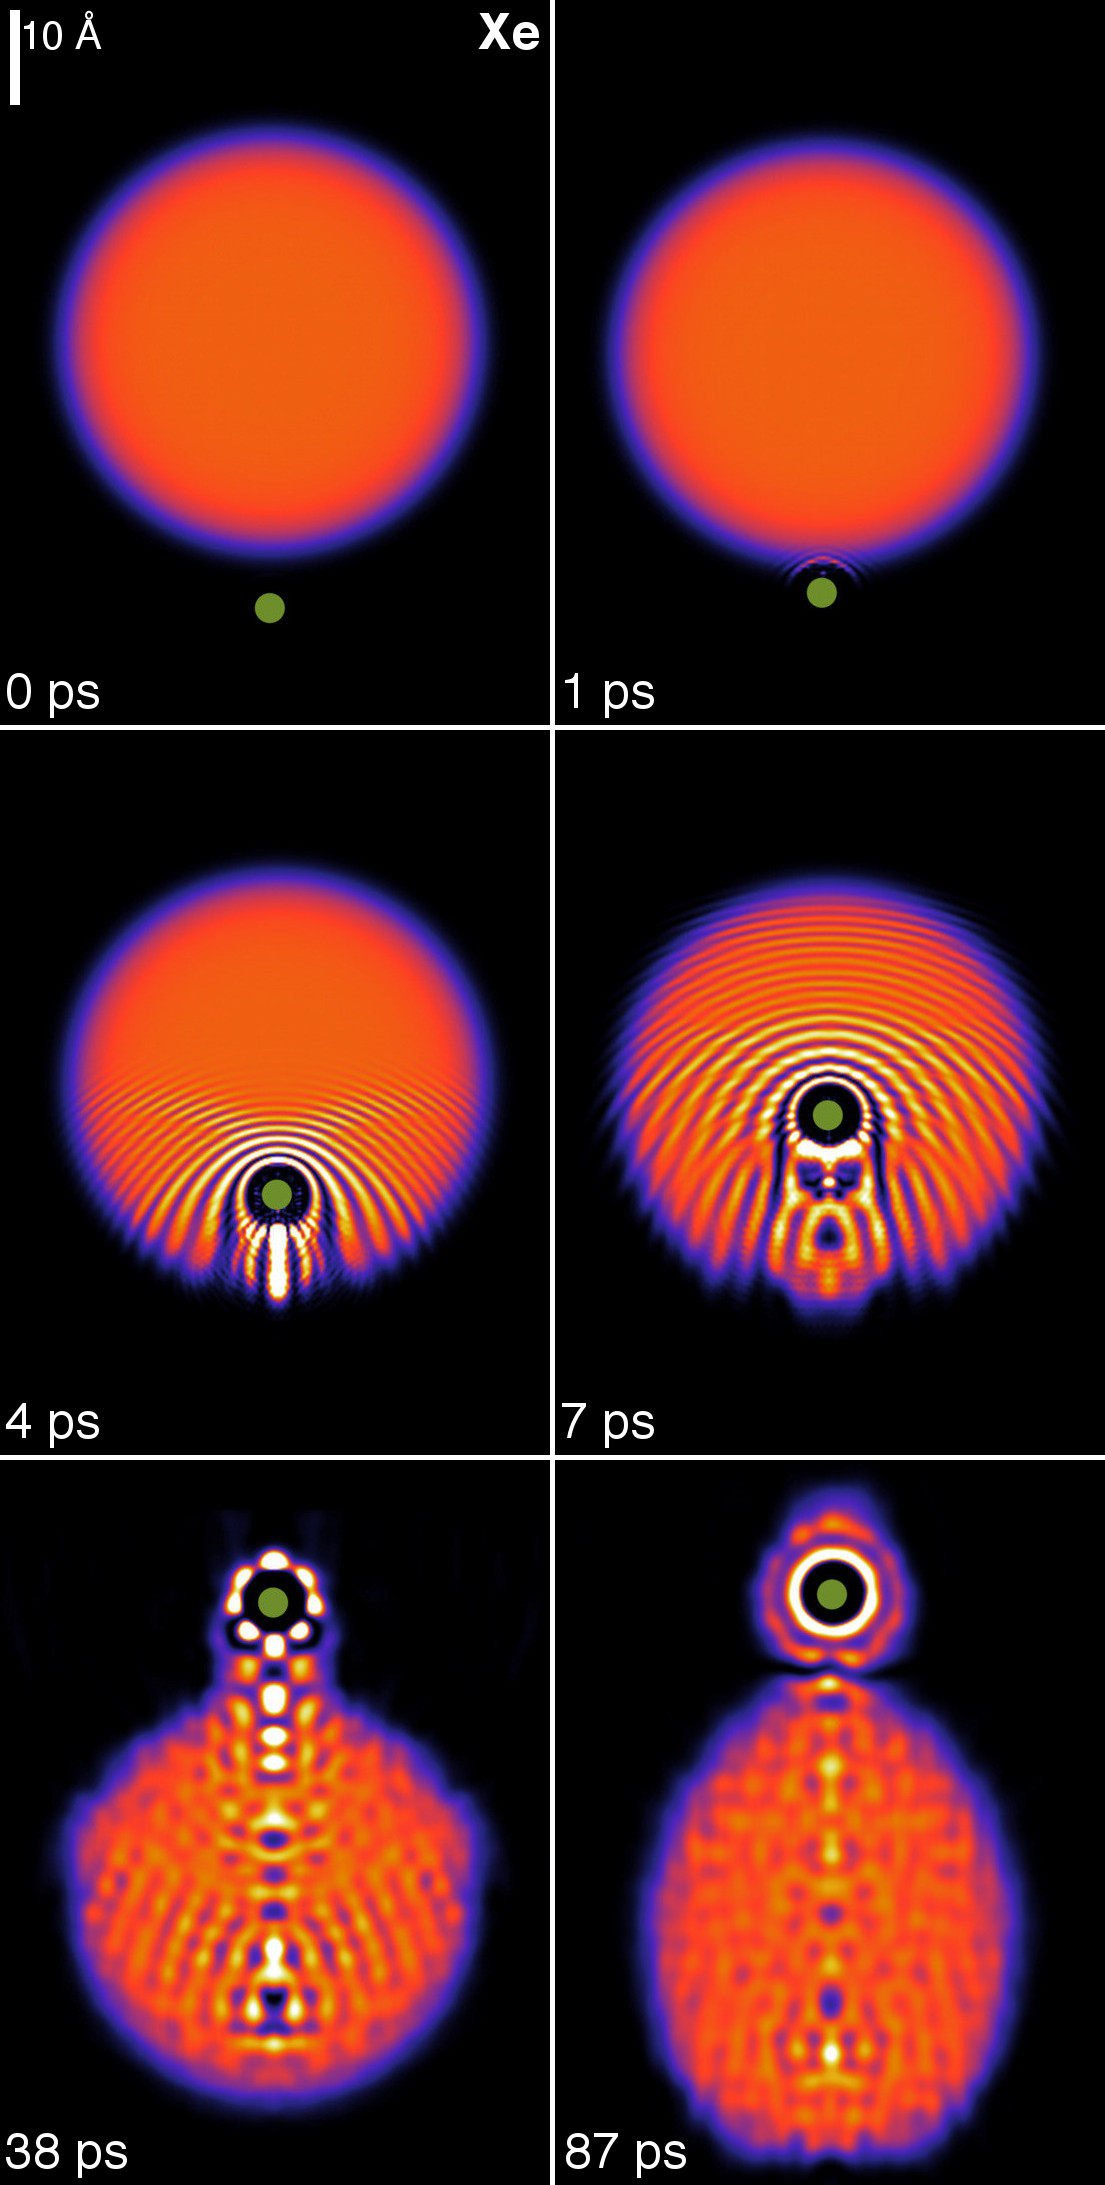
\includegraphics[width=0.6\linewidth,clip]{fig1-Xe-600mps}}
\caption{\label{fig1-capture} 
Dynamic evolution of a Xe atom (green dot) approaching the $^4$He$_{1000}$ 
droplet from below at $v_0 = 600$ m/s. The corresponding time is indicated in each frame. 
Bright spots correspond to high density regions. (Reproduced from\rf{Coppens2017-2}.)
}
\end{figure}
%

\begin{figure}[!]
\centerline{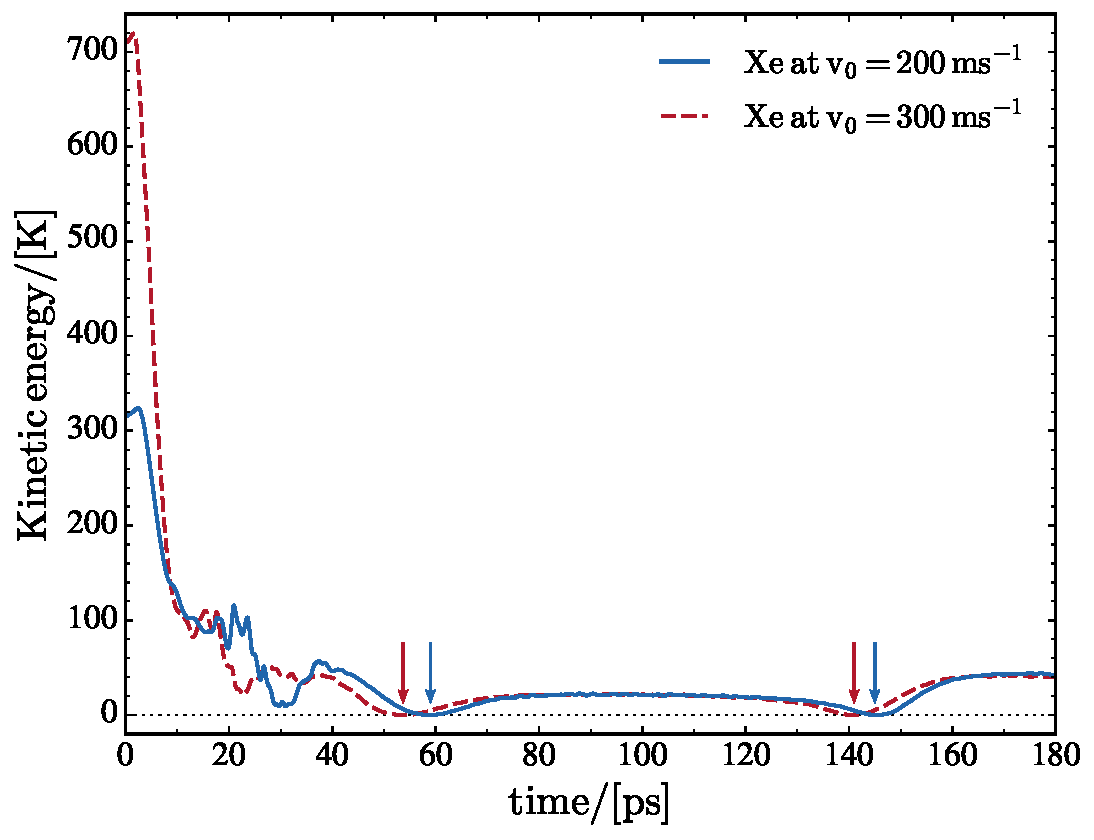
\includegraphics[width=0.9\linewidth,clip]{kinetic-energy}}
\caption{\label{fig2-capture} 
Kinetic  energy  of the Xe atom in the center of mass (COM) frame of the $^4$He$_{1000}$ droplet 
as a function of time for  a head-on collision  at $v_0$= 200 and 300 m/s. The kinetic energy increase 
during the first few picoseconds is due to the
acceleration produced by the attractive part of the Xe-He potential. The vertical arrows indicate the first two turning points inside the droplet.
}
\end{figure}
%
\begin{figure}[!]
\centerline{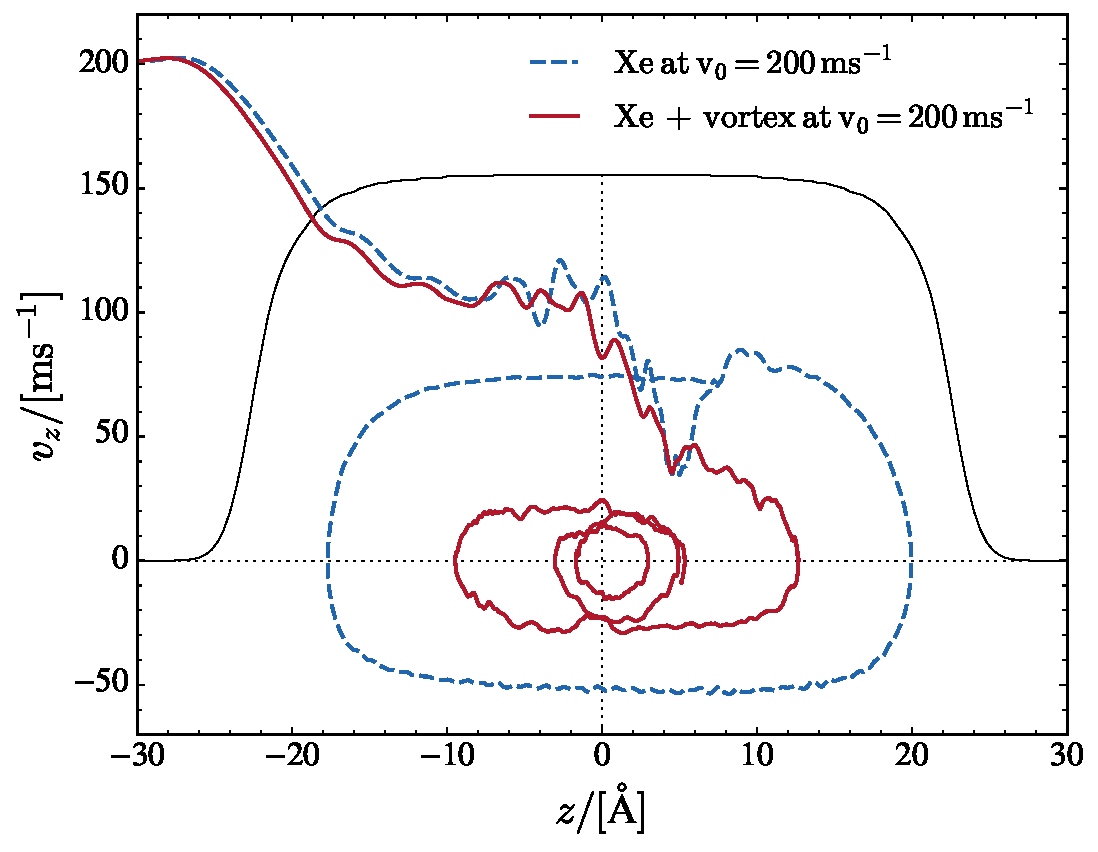
\includegraphics[width=0.9\linewidth,clip]{phase-Xe-200-vortex}}
\centerline{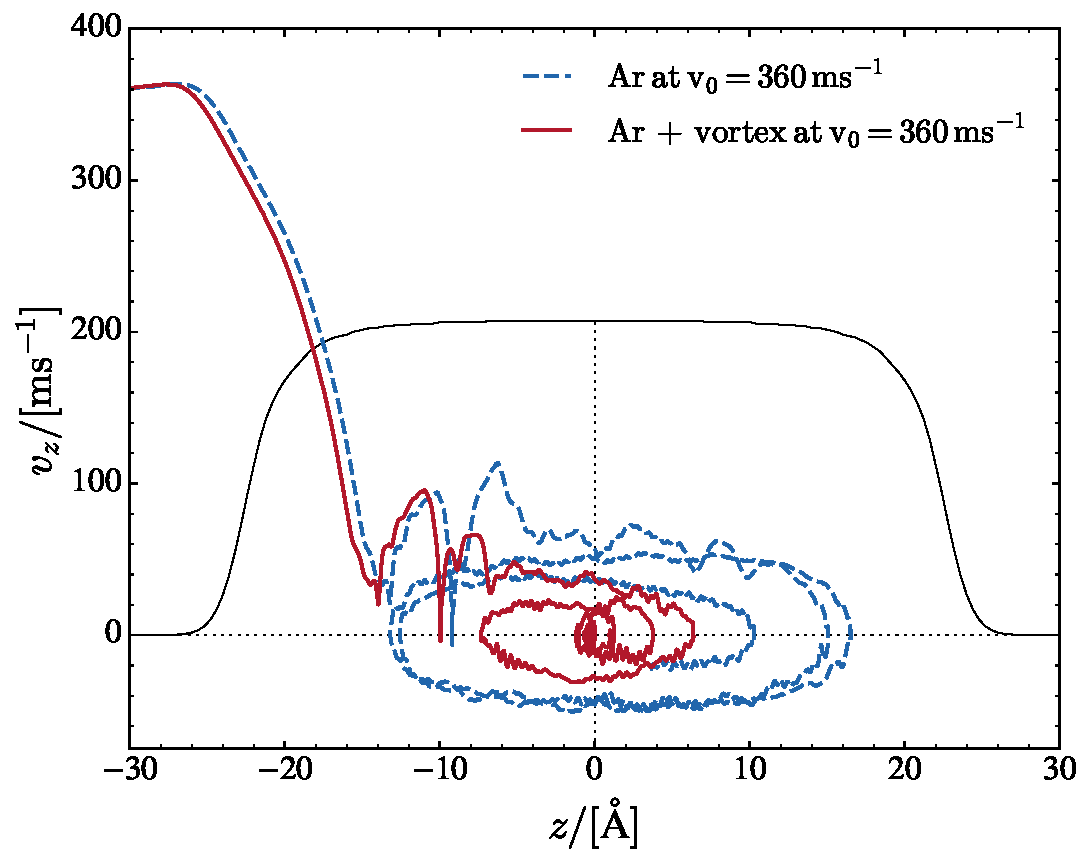
\includegraphics[width=0.9\linewidth,clip]{phase-Ar-360-vortex}}
\caption{\label{fig3-capture} 
Top: Phase-space trajectory  of Xe  for a  head-on collision at $v_0= 200$  m/s against a $^4$He$_{1000}$ droplet with and without a vortex line. 
The Xe atom is referred to the COM frame of the droplet.
Bottom: Same as top panel for Ar at $v_0=360$ m/s.
The droplet  density at $t=0$ is also represented in arbitrary scale (black profile) 
}
\end{figure}
%

%
\begin{figure}[!]
\centerline{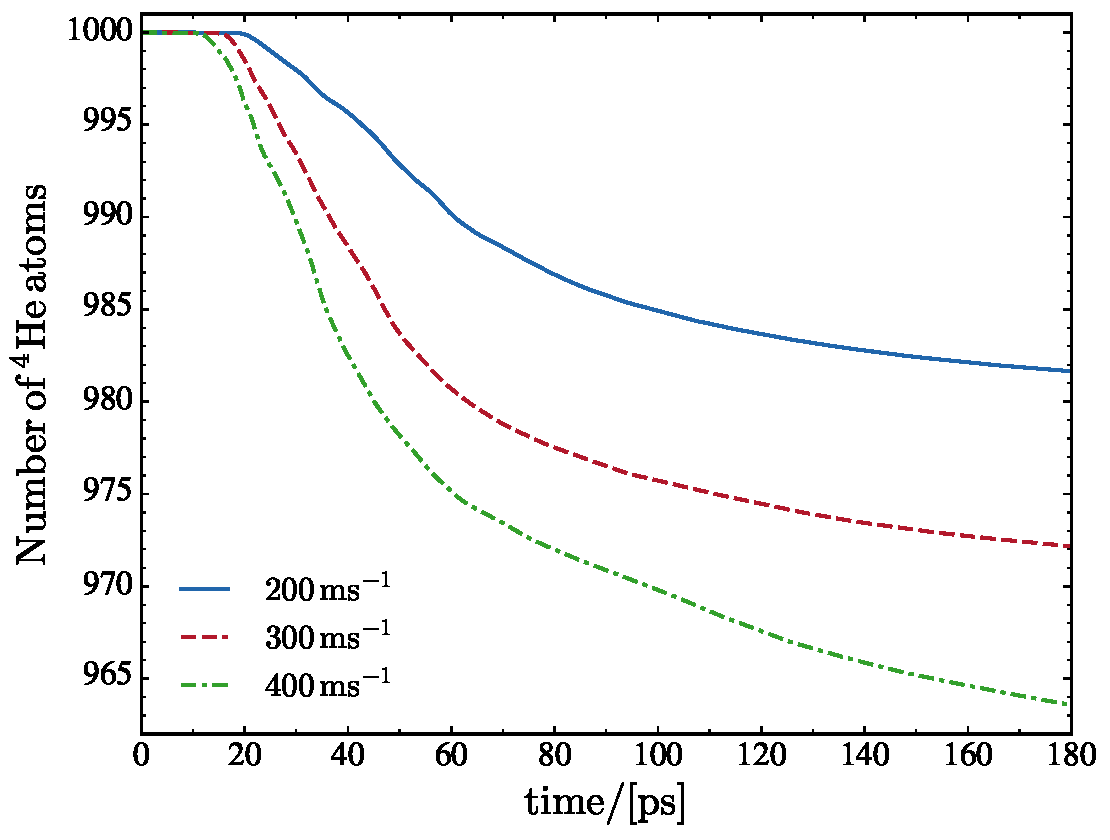
\includegraphics[width=0.9\linewidth,clip]{nparticles}}
\caption{\label{fig4-capture} 
Number of He atoms remaining in the droplet as a function of time for the
Xe against $^4$He$_{1000}$ collision at $v_0 = 200, 300$ and 400 m/s.
}
\end{figure}

We have simulated head-on collisions of a Xe atom with a
$^4$He$_{1000}$ droplet at relative velocities $v_0$ 
ranging from 200 to 600 m/s. \fig{fig1-capture} 
displays two-dimensional plots of the helium density 
for the highest value, $v_0= 600$ m/s. This velocity is 
well above the range of velocities typically encountered
in experiments\citep{Gom11,Gom14,Jones2016}.  
In spite of the appearance of disconnected helium density shown in the 
$t= 87$ ps frame, we have found that the Xe atom eventually 
turns around and is 
captured again inside the droplet even at that relatively high impact velocity. 
Note that the Xe impurity, even when it temporarily emerges from the bulk of the 
droplet, appears to be coated with a few
$^4$He atoms, see the configuration at 87 ps.

\fig{fig1-capture}  also shows the development of bow waves in the density profile, moving 
ahead of the impurity at 
supersonic velocity, and
an incipient  conic  density wave front  with its vertex at the Xe bubble.
Similar conic shapes, characteristic of supersonic flows, 
are found when an impurity moves in bulk liquid helium. 
In the present case the limited size of the droplet and 
the loss of kinetic energy
during the first stages of the collision
smooth out this front, making it just barely visible in the figure.

For low initial velocities of the impurity, we find that
Xe moves back and forth inside the droplet.
The turning points are not fixed,
because the droplet deforms due to the displacement 
of the Xe atom and to the waves that are continuously emitted 
by the moving impurity
(mainly in the direction of its  motion),
hit the droplet surface, and are reflected back inside it\citep{Coppens2017-1}.
This is shown in 
\fig{fig2-capture} for $v_0= 200$  and 300 m/s. 
Thermal Xe atoms ($v_0 \sim$ 240 m/s) 
are used in the vortex imaging 
experiments\citep{Gom14,Jones2016}, and the average droplet velocity 
as it travels through the pick-up chamber is about 
170 m/s\citep{Gom11}, corresponding to relative collision
velocities which are within the range investigated here.
The kinetic energy gained by the Xe atom 
after the turning point at 140 --150 ps
is precisely due to the fact that the droplet is not a rigid 
object and reacts to the motion of the impurity.
As a consequence, energy is transferred not only from the impurity to 
the droplet but also the other way around. 
%A similar effect 
%was found in the sinking of a Ba$^+$ cation,
%see the multimedia view indicated in the caption of Fig. 2 of  ref. \citep{Mat14}
We want to emphasize that the droplet experiences 
large deformations rather than 
large displacements;
the velocity of the center of mass (COM) of the droplet is 
rather small (below 6 m/s  for $v_0= 200$ and 300 m/s as well) 
due to the large 
mass difference between the impurity and the droplet.

We have found that most of the energy is transferred from 
the Xe to the droplet in the first stages of the collision.
This is why, for collisions in this kinetic energy range 
leading to Xe capture, the motion of the impurity inside the droplet
is independent on the initial kinetic energy to a large extent.  
This is shown in \fig{fig3-capture}, which displays the trajectory
of Xe (Ar) in phase space for $v_0= 200$ (360) m/s. 
The figure also shows similar trajectories in the case where a vortex 
is present in the droplet; these cases will be discussed later in this paper.

\begin{table}
	\caption{\label{tab1} Number of He atoms promptly ejected ($N_e$) and average energy per ejected atom ($E_e$) during the first 200 ps.}
	\taburulecolor{activeColor}
	\begin{tabu} to \textwidth {X[c]X[c]X[c]X[c]}
		\toprule
		Species & $v_0$~(m/s) & $N_e$ & $E_e$~(K) \\
		\midrule
		Xe & 200 & 18 & 19 \\
		& 300 & 28 & 23   \\
		& 400 & 37 & 30 \\
		\midrule
		Ar & 360 & 16 & 22 \\
		\bottomrule 
	\end{tabu}
\end{table}

The kinetic energy lost by the impurity atom is partly deposited 
in the droplet, where it produces large deformations and sound waves, 
and partly carried away by   prompt-emitted helium atoms. These are atoms  with a 
significant kinetic energy which are expelled from the droplet  
early on in the collision process. 
%A similar ejection appears in nuclear heavy ion reactions at intermediate energies, see e.g. ref. \citep{Ler85}
%and references therein.  
\fig{fig4-capture}   shows the number of atoms remaining in the simulation cell as a function of time
for collisions with Xe at $v_0= 200, 300 $ and 400 m/s. 
Eventually, the energy deposited into the droplet should be lost by atom evaporation.
The energy carried away by the ejected He atoms during the first 200 ps is 
collected in \tab{tab1} for the head-on collisions described in this paper.
For comparison, the  calculated binding energy of  a helium atom in the $^4$He$_{1000}$ droplet is $6.0$ K.
Note that helium atom ejection continues after 200 ps, the droplet still being far from ``thermalized'' (equilibrated).

In the case of heavy dopants it is possible to obtain 
a simple expression for their capture cross 
section.  Defining
%
\begin{equation}
\kappa=\sqrt{\frac{2 \mu E}{\hbar^2}} \;\; ,
\label{eq9}
\end{equation}
%
where $\mu$ is the reduced mass of the system and
$E$ is the available energy in the center-of-mass frame, and 
provided that the reduced de Broglie wave length of the impurity
$\lambda/(2 \pi) = 1/\kappa$ is much smaller than the dimensions 
of the droplet (which is the case for all $v_0$  in this study), the system
behaves classically and\citep{Lea14a}
%
\begin{equation}
\sigma(E)= \frac{\pi}{\kappa^2 } \sum_{\ell=0}^{\ell_{cr}} (2 \ell
+1)= \frac{\pi}{\kappa^2 } (\ell_{cr} +1)^2  
\label{eq10}
\end{equation}
%
where $\ell_{cr}$ is the largest relative angular momentum leading to the impurity capture. 
For a given energy, $\ell_{cr}$ is determined by 
carrying out simulations with different impact parameters $b$ using  
$\ell= \mu v_0 \, b/\hbar$.
We have done it for Xe at $v_0= 200$ m/s. \fig{fig5-capture} shows the 
simulation corresponding to the largest impact parameter among the ones we have calculated
which led to Xe capture, $b=20.3$ \AA{}, and
\fig{fig6-capture} shows the simulation corresponding to the smallest one
which led to Xe deflection, $b=22.2$ \AA{}.
The radius of the 
droplet, which is defined as $R= r_0 N^{1/3}$ 
with $r_0 = 2.22$ \AA{}, is 22.2 \AA{} for $N=1000$. 
Hence, at this energy --well within the thermal conditions of the experiment--
the cross section for Xe capture is very similar to the geometric droplet cross section. 

 The circulation lines of the superflow are displayed 
in two selected panels in \fig{fig5-capture} and \fig{fig6-capture}. 
They show the flow  pointing towards
the approaching Xe atom at the beginning of the collision and the appearance of vortex loops  
in the droplet at the latest stages of the simulation.
Vortex loops appear  from local distortions of the droplet surface\citep{Lea14b}. 
%They have been found in other processes, such as the sinking of Cs$^+$ and Rb$^+$ cations in helium droplets.\citep{Lea14b}
%The motion of an impurity inside a droplet  has also been found to lead to vortex ring nucleation.\citep{Mat14} 
%It is unclear to us why sometimes  vortex rings are nucleated and sometimes not.
%We mention that 
The circulation lines  displayed  in the figures of this work have been drawn inside the region where the density is above  0.5 $\rho_0$ (with $\rho_0$= 0.0218 \AA$^{-3}$)
 that defines the dividing surface of the droplet. 

\begin{figure}[h]
\centerline{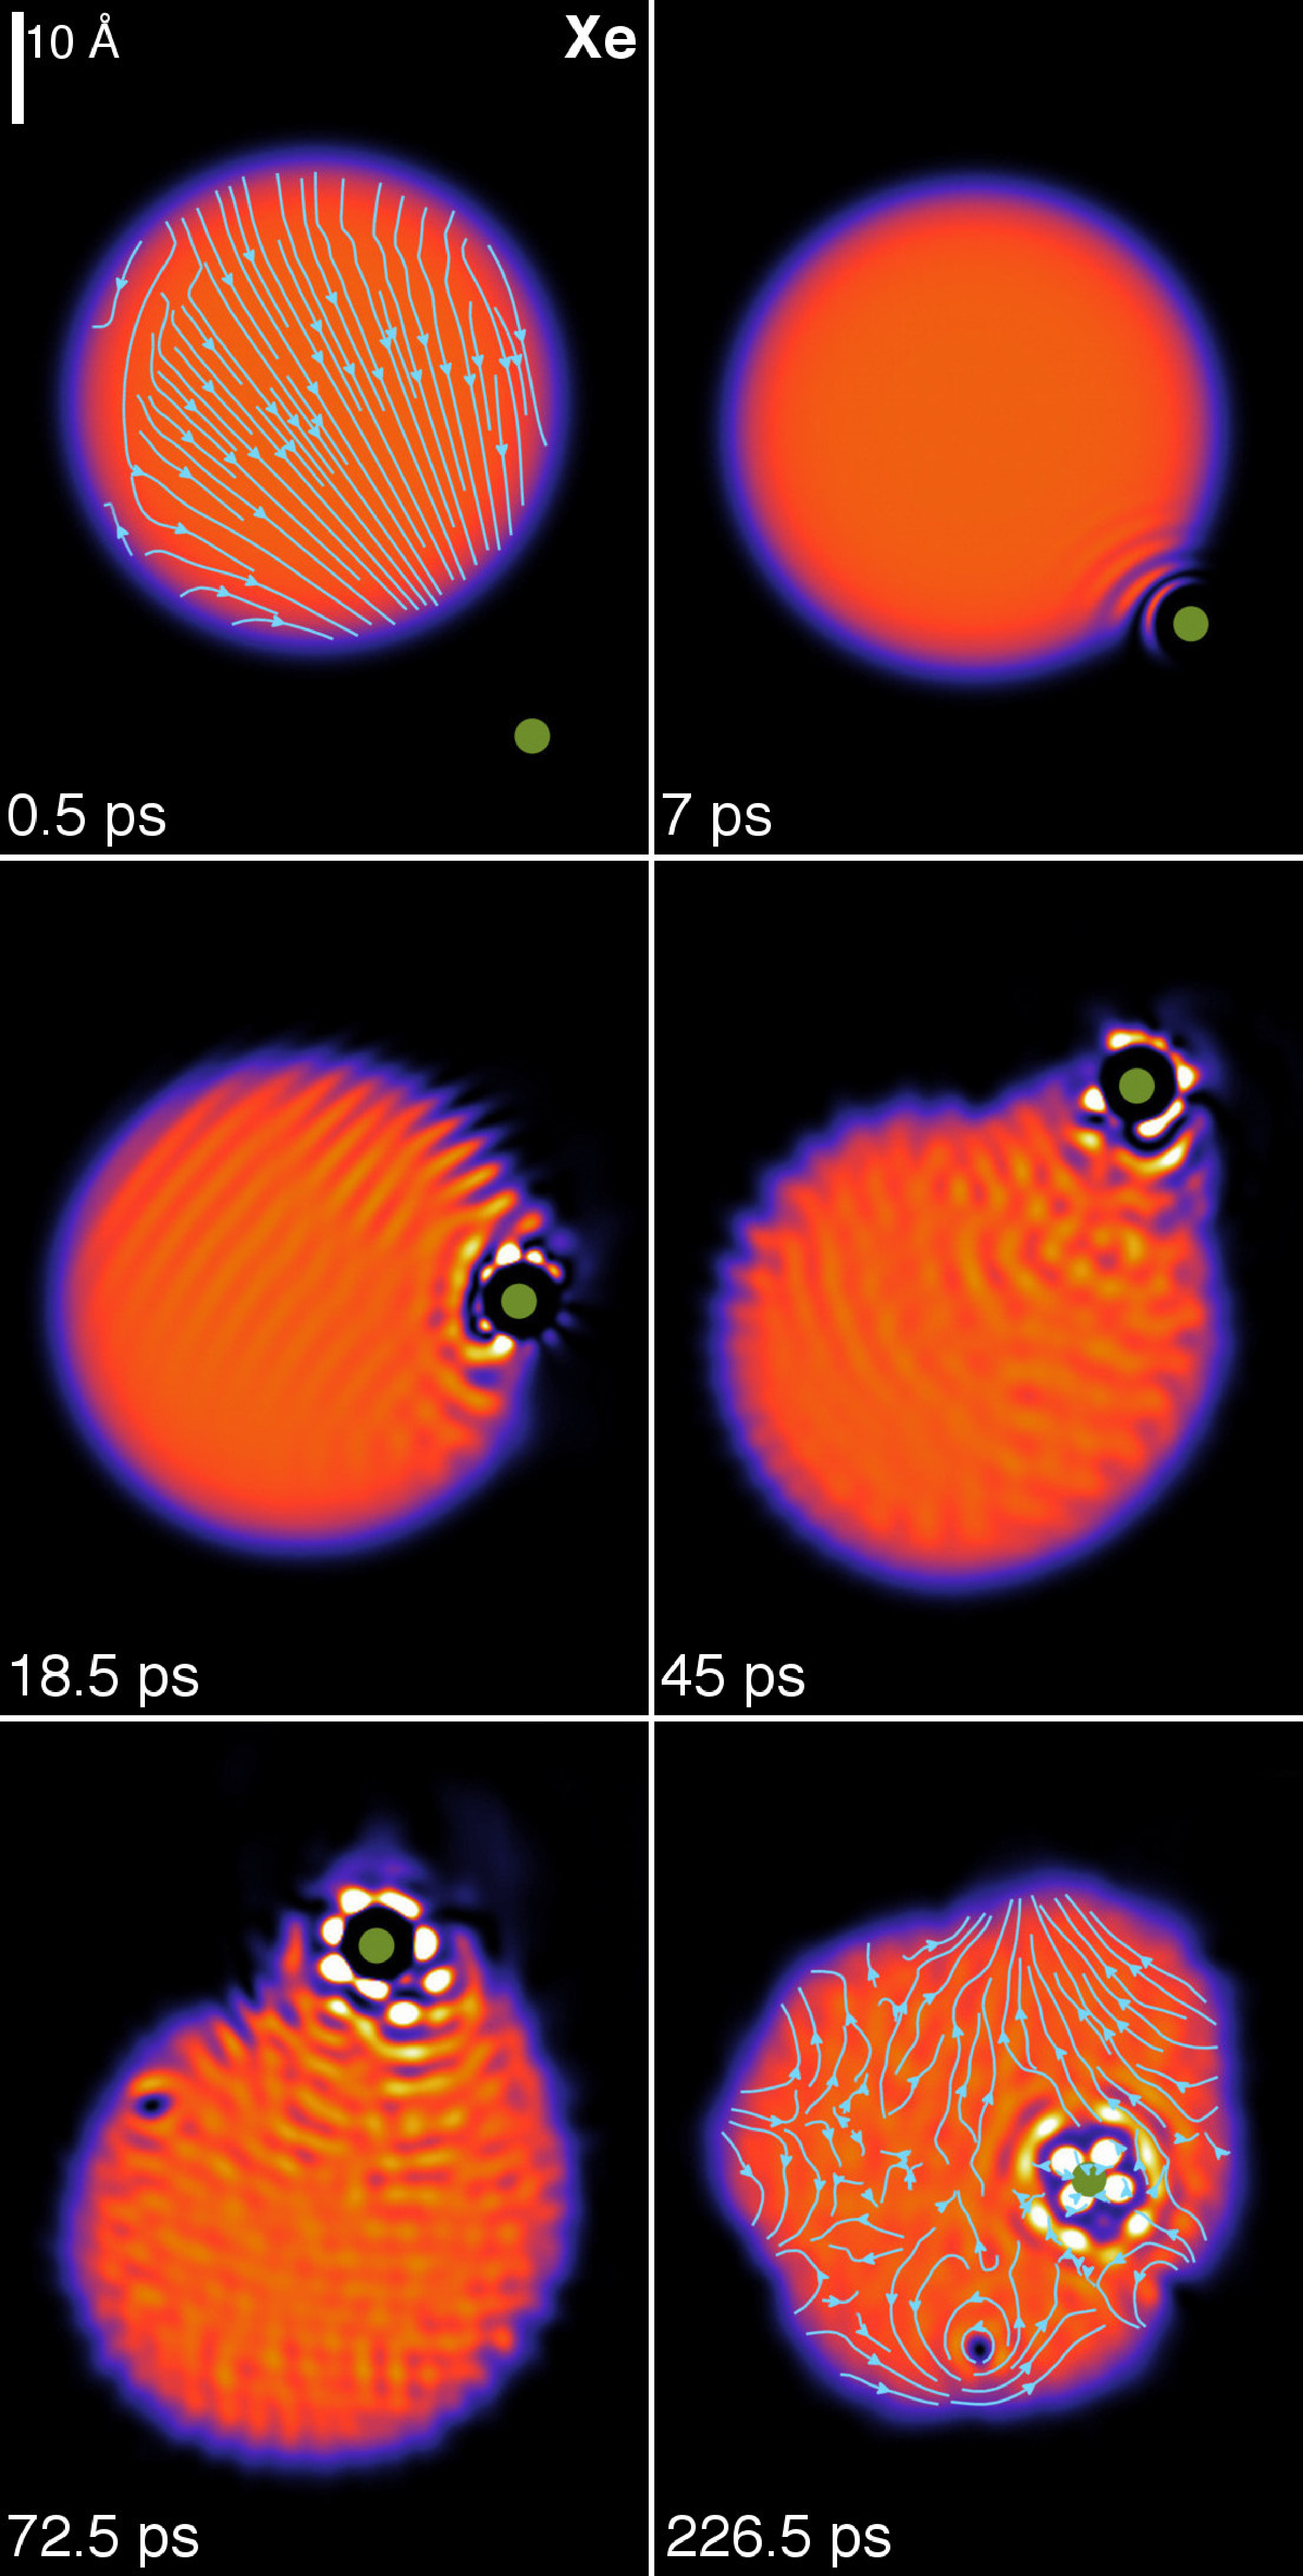
\includegraphics[width=0.60\linewidth,clip]{xehe200-b203-composed}}
\caption{\label{fig5-capture} 
Dynamic evolution of a Xe atom (green dot) approaching the $^4$He$_{1000}$ 
droplet from below at $v_0 = 200$ m/s with impact parameter $b = 20.3$ \AA{}. The corresponding time is indicated in each frame. The velocity fields are represented in cyan in the panels at 0.5~ps and 226.5~ps. The bright spots are high He density blobs appearing around the Xe atom because of the attractive He-Xe interaction. See the ESI\citep{Coppens2017-2} for the movie of the complete evolution. 
}
\end{figure}
%

\begin{figure}[h]
\centerline{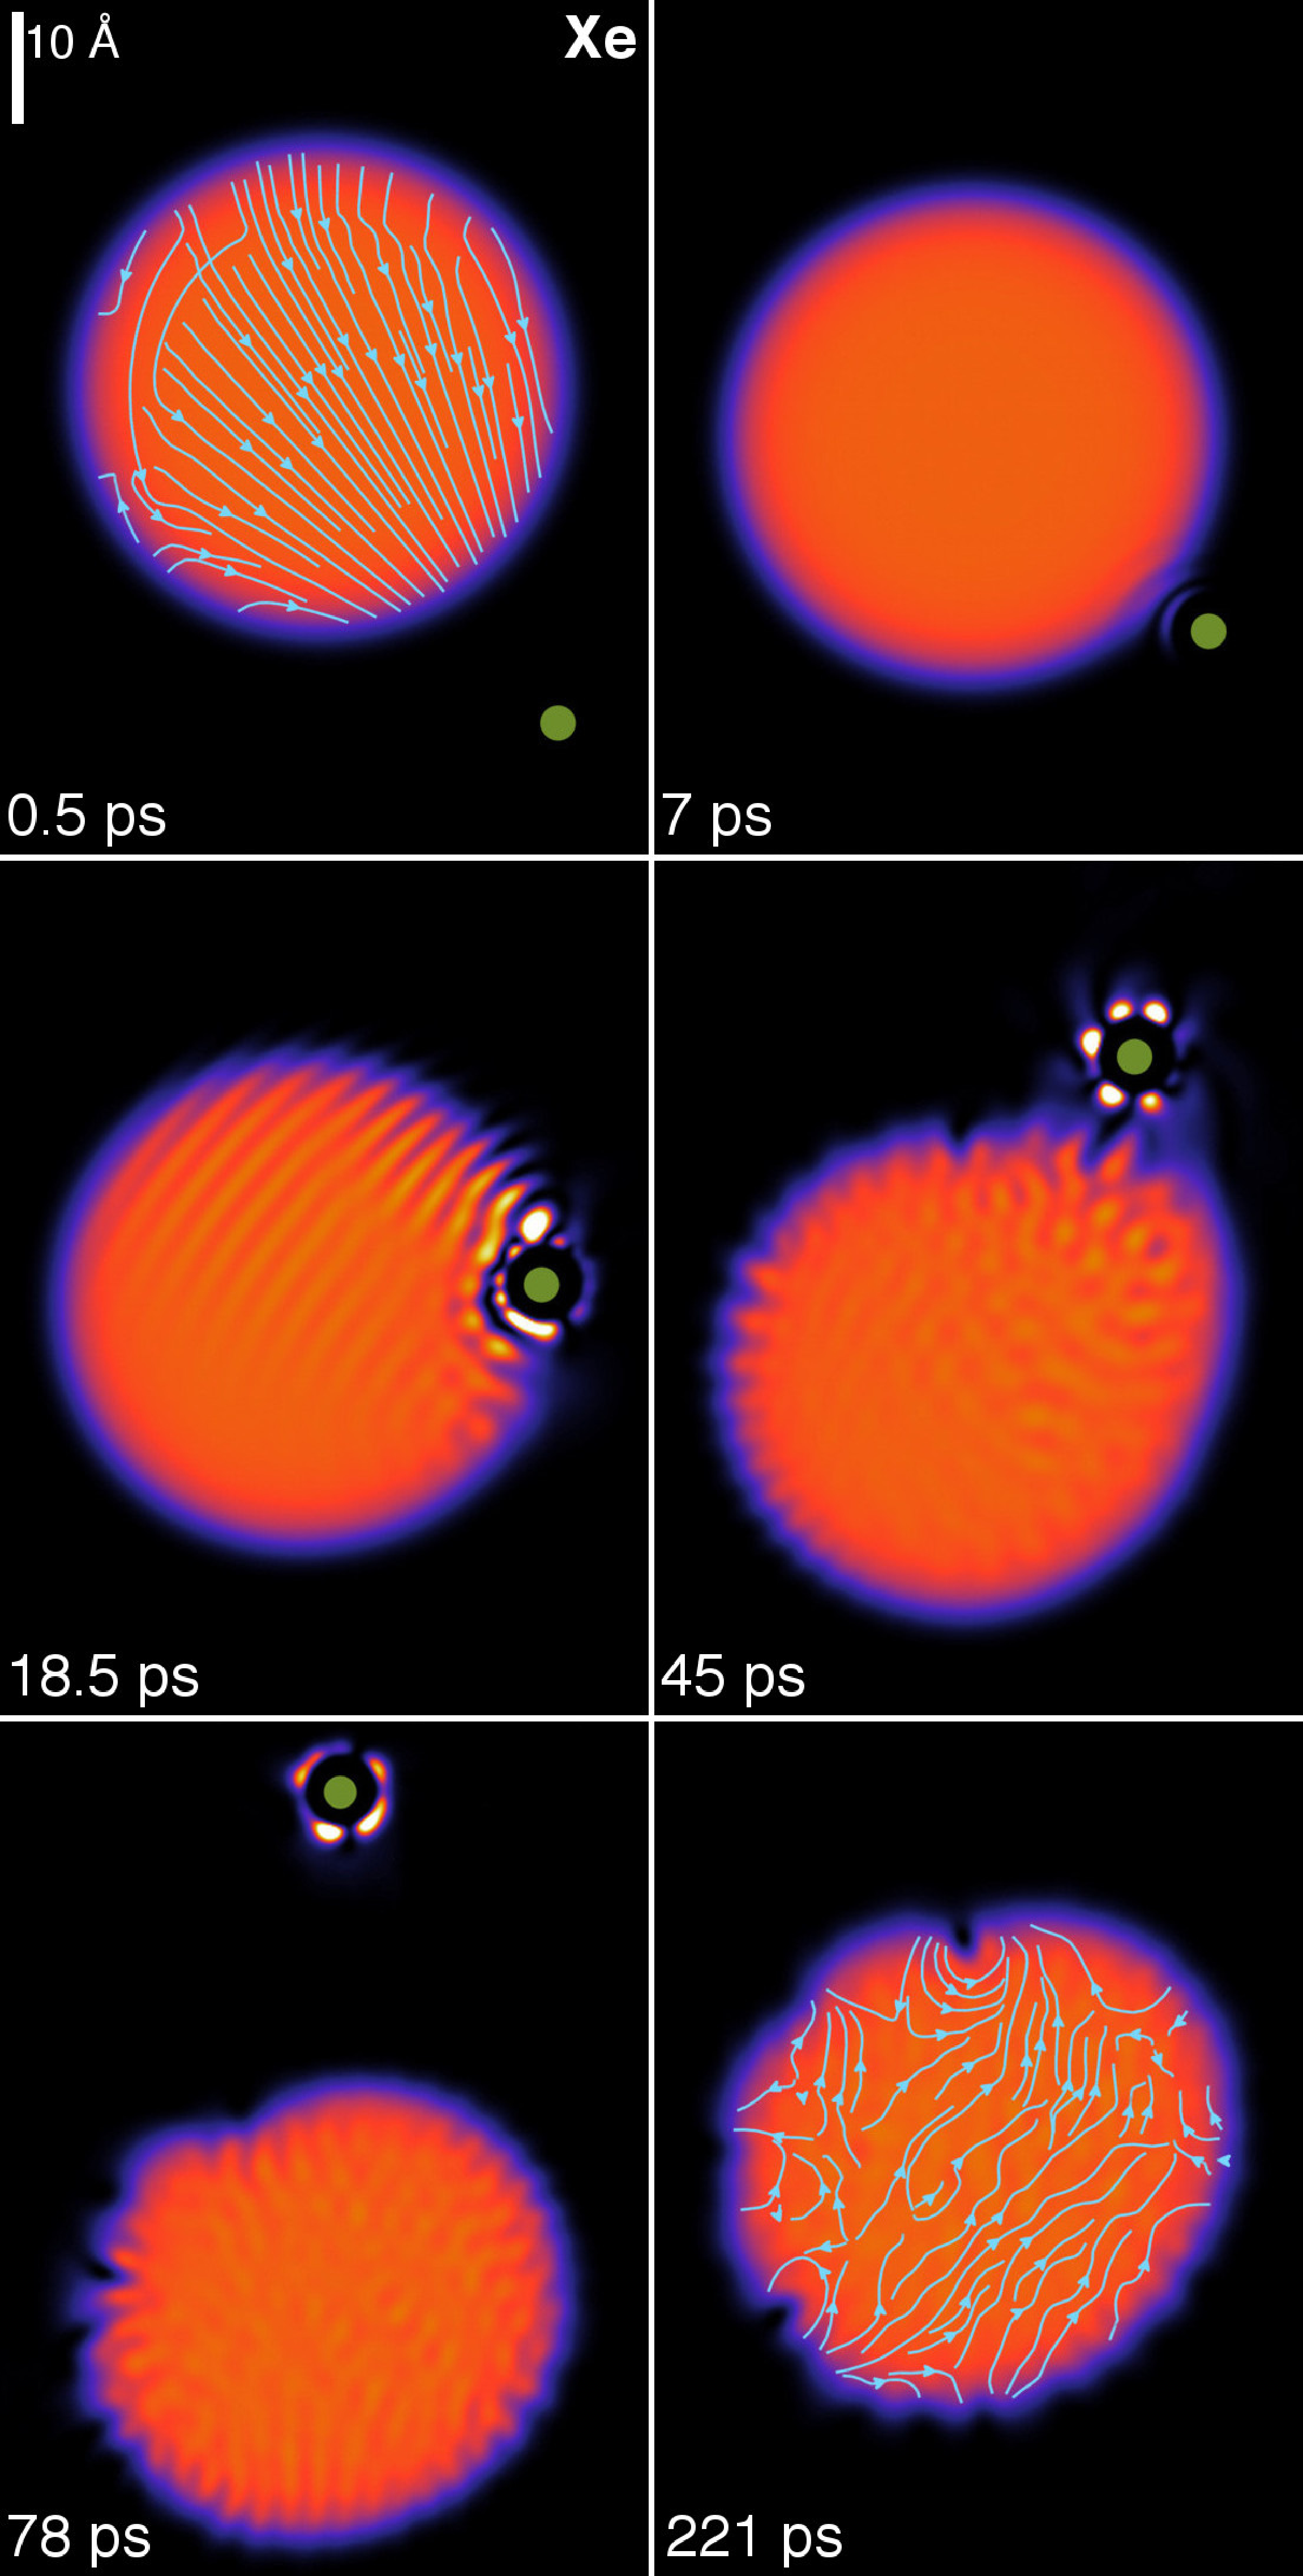
\includegraphics[width=0.60\linewidth,clip]{xehe200-b222-composed}}
\caption{\label{fig6-capture} 
The same process as in \fig{fig5-capture} but with an impact parameter $b = 22.2$~\AA{} instead of $b = 20.3$~\AA{}. Note that in this case, after about 78~ps (bottom left panel), the Xe atom is ejected with some helium density attached to it. See the ESI\citep{Coppens2017-2} for the movie of the complete evolution.   
}
\end{figure}
%

In peripheral collisions not only energy but also angular momentum 
is deposited into the droplet, which allows  
to visualize the  irrotational flow of the superfluid helium.
In particular,
for Xe at $v_0=$200 m/s and $b$=22.2~\AA{} the initial angular momentum is 917 $\hbar$. 
This collision was followed for some 220 ps and
produced the ejection of 15 He atoms, 5 of them attached to the Xe atom, see \fig{fig6-capture}. 
After the collision, the Xe+$^4$He$_5$ complex carries away 522 
angular momentum units, while some 95 units are deposited in the droplet as vortex loops and
capillary waves\citep{Whitaker1998}, see bottom right panel of \fig{fig5-capture} and \fig{fig6-capture}. 
The remaining angular momentum is taken away by the ejected helium atoms.

\section{Helium droplets hosting vortex lines}\label{sec:vtx-lines}

To determine the structure of a droplet hosting a singly-quantized linear vortex 
we have started the imaginary time iteration from a helium  
density in which the vortex is ``imprinted''. For this purpose, a vortex line
along the $z$  can be described by the effective wave function 
%
\begin{equation}
\Psi_0(\mathbf{r}) =  \rho_0^{1/2}(r) \, e^{i  \, {\cal S}(\mathbf{r})} = \rho_0^{1/2}(\mathbf{r}) \, \frac{(x + i y)}{\sqrt{x^2 + y^2}} 
\label{eq11}
\end{equation}
%
where $\rho_0(\mathbf{r})$ is the density of 
either the pure or  the impurity-doped droplet without vortex.  
Vortex lines along other directions passing through a chosen point 
can be imprinted as well\citep{Pi07}.
%;  more involved imprinted configurations can be found {\it e.g.} in ref. \citep{Pi07}. 
 
In the case represented by \eq{eq11}, if the impurity is within the vortex
core along a symmetry axis of the impurity-droplet complex,
the effective wave function $\Psi_0({\mathbf r})$ -- before and after relaxation -- is an eigenvector of the  angular 
momentum operator  $\hat{L}_z = -i \; \hbar \partial/\partial \theta$. 
The angular momentum of the droplet is then
 %
\begin{equation}
\langle \hat{L}_z \rangle = \langle \Psi_0(\mathbf{r}) | \hat{L}_z  | \Psi_0(\mathbf{r}) \rangle = N \; \hbar
\label{eq12}
\end{equation}
%

%As far as the energetics of the impurity-droplet-vortex complex is concerned, 
Different energy balances involving pure and doped droplets 
hosting vortices are defined\citep{Pi07,Anc15,Dal00}:
%
\begin{itemize}
\item
Solvation energy of the impurity:

$ S_X = E(X@^4{\rm He}_N) - E(^4{\rm He}_N)$

\item
Vortex  energy:

$E_V= E(V@^4{\rm He}_N) - E(^4{\rm He}_N)$

\item
Binding energy of the impurity to the vortex: 

$B_X = S_X - \{E[(X+V)@^4{\rm He}_N] - E(V@^4{\rm He}_N)\}$

\end{itemize}
%
Using the functional of\rf{Anc05a} and the He-rare gas pair potentials of\rf{Tan86}, solvation energies
of  -316.3 K and -215.7 K have been  found for Xe and Ar atoms, respectively. Thus, for the same incident kinetic
energy, about 100 K of additional energy have to be dissipated in the case of Xe in order to get the same kinematic conditions than for Ar.

The  binding energy of the impurity to the vortex
is the result of a delicate balance between terms which are
individually much larger than
their difference. It can thus be affected by relatively 
large inaccuracies.
Within DFT, it has been found that the Xe atom
 is barely bound to the vortex line, with $B_{Xe}\sim 3-5$ K\citep{Dal00,Anc14}.

%The kinetic energy of the superfluid flow in the volume excluded by the
%impurity intuitively corresponds to $B_X$. For this reason, $B_X$ is 
%also called  ``substitution energy''.\citep{Don91}
%Using a sharp helium density model for the impurity 
%bubble and the vortex line, it can be shown that\citep{Don91}
%
%\begin{eqnarray}
%&&B_X = 2 \pi \frac{\hbar^2}{m_4} \rho_0  \,R_X \times 
%\\
%\nonumber
%&&
%\left\{\left(1 +  \frac{a^2}{R_X^2}\right)^{1/2} 
%\,ln \left[\frac{R_X}{a} + \sqrt{\left(\frac{R_X}{a}\right)^2+1}\right] - 1 \right\} \; ,
%\label{eq13}
%\end{eqnarray}
%
%where $a$ is the radius of the vortex core and $R_X$ is the radius of the atomic bubble.
%Taking $\rho_0= 0.0218$ \AA$^{-3}${}, $a=1$ \AA{} and $R_X=3.5$ \AA{},  
%which corresponds to the value where the Xe-He pair potential becomes repulsive,
%one obtains $B_{Xe}= 6.1$ K. In the case of Ar, $R_X$=3.1 \AA{} and $B_{Ar}$=4.8 K.

A critical angular velocity $\omega_c$ exists above which nucleation of
vortices with quantized velocity circulation in units of $h/m_4$ occurs.
The critical angular velocity for nucleating a vortex line  along a diameter
in a droplet made of $N$ helium atoms is
%
\begin{equation}
\omega_c  = \frac{1}{\hbar}\,\frac{E_V}{N} 
\label{eq14}
\end{equation}
%
This expression is obtained by computing the energy that 
minimizes $\langle H -\omega L_z\rangle$ ({\it i.e.} corresponding 
to the equilibrium configuration in the corotating frame) with and without 
a vortex line\citep{Dal96}.
% 
Using the values appropriate for a $^4$He$_{1000}$ 
droplet we obtain $\omega_c =  0.127$ K/$\hbar$ = 0.0167\,  ps$^{-1}$.

%The velocity field corresponding to axially symmetric configurations with one vortex along the $z$-axis is
%
%$$ \mathbf{v}(\mathbf{r}) = \frac{\hbar}{m_4} \frac{1}{r} \hat{\theta}$$
%
%where $r$ is the distance to the $z$-axis and 
%$\hat{\theta}$ the unit vector in 
%the increasing $\theta$ direction (counterclockwise);
%the circulation lines on the $x-y$ plane  are circumferences.\citep{Don91} 
%It is worth mentioning that the above velocity field 
%is irrotational, but this is not the only possibility. 
%Indeed, below $\omega_c$ the superfluid droplet may store
%some angular momentum smaller than $\hbar N$ without 
%hosting any vortex; the only constraint is that 
%the velocity field of the superfluid must be irrotational. 
%We will come back to this point later on.

When the angular velocity is increased 
above $\omega_c$, larger amounts of angular momentum may be stored
into the superfluid by increasing the number of 
nucleated vortices. The higher the angular velocity,  
the more packed the vortex array is
around the rotation axis.  
These vortices arrange themselves into ordered structures  
whose existence in bulk superfluid $^4$He was established long ago\citep{Vin61,Wil74}.

To generate vortex arrays we have worked in the  
fixed-droplet frame of reference (corotating frame at  
angular velocity $\omega$), {\it i.e.} we look for solutions of the following EL equation: 
%
\begin{equation}
\{{\cal H}[\rho] \,-\omega \,\hat{L}_z\} \,\Psi(\mathbf{r})  =  \,\mu_4 \,
\Psi(\mathbf{r}) \;,
\label{eq15}
\end{equation}
%
In this case, $\Psi(\mathbf{r})$ no longer is  
an eigenvector of the angular momentum.
To determine $\Psi(\mathbf{r})$ describing a 
configuration where $n_v$ vortex lines are present we have followed 
again the imprinting strategy, starting the imaginary-time evolution of  
\eq{eq15} with the helium effective wave function
%
\begin{equation}
\Psi_0(\mathbf{r})=\rho_0^{1/2}(\mathbf{r})\, \prod _{j=1}^{n_v} \left[ {(x-x_j)+i (y-y_j) \over \sqrt{(x-x_j)^2+(y-y_j)^2}}  \right] 
\label{eq16}
\end{equation}
%
where  $\rho_0(\mathbf{r})$ is the density of the vortex-free 
droplet and $(x_j, y_j)$ is the initial position of the $j$-vortex linear  core with
respect to the $z$-axis of the droplet (note that in\rfs{Anc14,Anc15} $\Psi_0(\mathbf{r})$ was incorrectly written).
We underline the fact that during the functional minimization 
of the total energy, the vortex positions and shapes will change
to provide at convergence the lowest energy vortex 
configuration for the given value of the angular velocity $\omega$.  

\begin{figure}[h]
\centerline{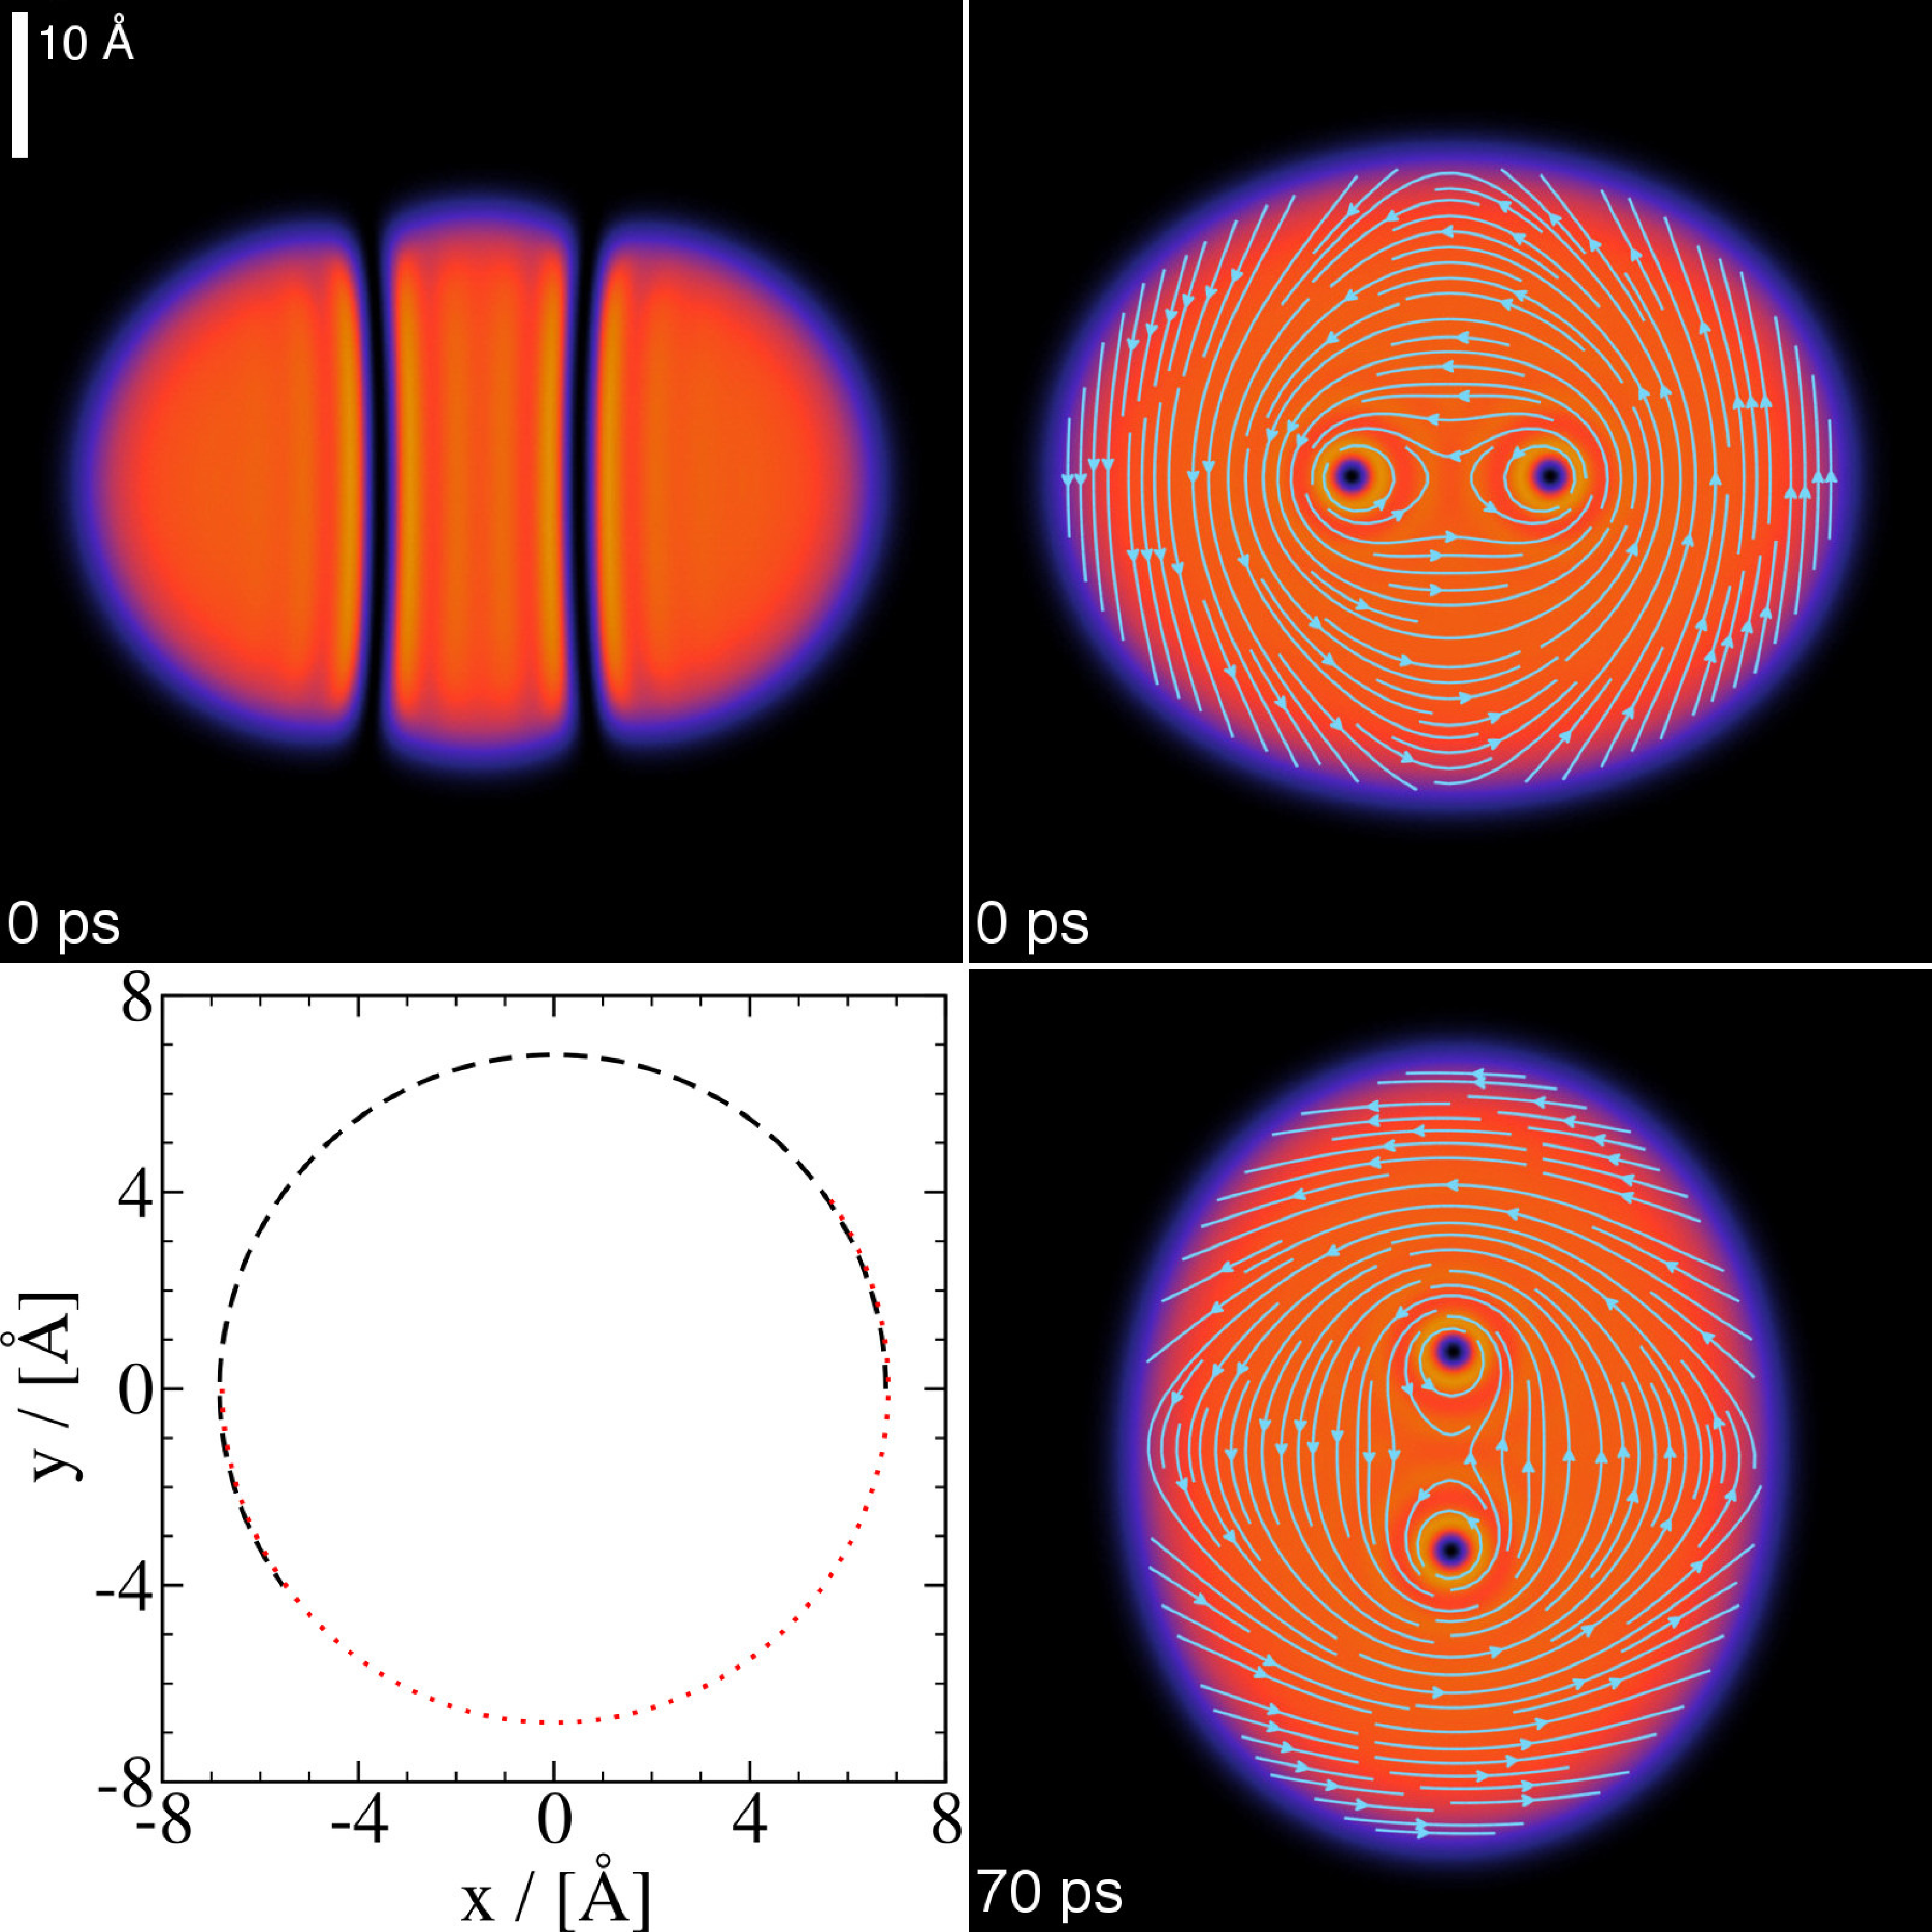
\includegraphics[width=0.8\linewidth,clip]{fig7}}
\caption{\label{fig7-capture}
$^4$He$_{1000}$ droplet at $\omega= 0.0229$ ps$^{-1}$: Top panels, stationary 
two-vortex configuration on the $x-z$ plane (left) and  $x-y$ plane (right)  in the corotating frame.
Bottom left panel, trajectory of the vortex cores 
in the $x-y$ plane of the laboratory frame. 
The dashed line is the trajectory of one of the vortex cores, and the dotted line that of the other. Both trajectories  overlap and show that the vortex cores rotate rigidly and this is also visualised by the velocity field lines shown in the right two panels. xBottom right panel, helium density in the $x-y$ plane at $t=70$ ps obtained in the laboratory frame starting from the above configuration\citep{Coppens2017-2}. 
}
\end{figure}

\fig{fig7-capture} shows the two-vortex  
stationary configuration of a $^4$He$_{1000}$ droplet  in the corotating frame 
at angular frequency $\omega$= 0.175 K/\,$\hbar=$ 0.0229 ps$^{-1}$. 
The angular momentum  of this configuration is  $\langle \hat{L}_z \rangle = 1836 \; \hbar$. 
Notice the bending 
of the vortex line so that they meet  
the droplet surface perpendicularly at both ends, and also the 
flattening of the droplet in the $z$ direction
due to centrifugal forces.

At variance with the single vortex line along the symmetry 
axis of the droplet, the two-vortex  configuration is not stationary in the laboratory frame, 
where the density and velocity field change with time. 
To show this, $\Psi(\mathbf{r})$ has been evolved 
in the laboratory  for about 150 ps
taking as initial condition the stationary 
configuration in the corotating frame. 
As expected, the vortex cores appear to rotate in the laboratory frame. 
Within the numerical accuracy, they do so rigidly. This can be seen in 
\fig{fig7-capture}. Besides, they rotate precisely at 
$\omega$= 0.0229 ps$^{-1}$. This is a  stringent test 
on the accuracy of the dynamics and the consistency of the method.
It can be seen in the ESI 
material how  the two vortex lines turn around each other.

\fig{fig7-capture} shows how a superfluid droplet 
hosting a vortex array ``rotates''. The fact that the vortex 
cores rotate rigidly is not in 
contradiction with the irrotational character 
of the superfluid flow, since they are empty.  The cores carry 
along with them the superfluid whose velocity field  is irrotational,
whereas for a rigid solid or a classical liquid in steady flow 
 one has $\mathbf{v} = \omega \times \mathbf{r}$,  hence $\nabla \times \mathbf{v} = 2\, \omega$. 
The circulation lines in \fig{fig7-capture} do not correspond 
to a rigid rotation, but to  an irrotational flow in the presence of two vortices. 
The helium density adapts to the vortex cores as they 
rotate and this gives the appearance of a solid 
rotation in the laboratory frame, but it is not. 

It is worth discussing the different  configurations 
that may appear when $\omega < \omega_c$. The lowest energy  
corresponds to the current-free ($CF$) $\langle L_z \rangle =0$ configuration. 
Metastable one-vortex ($1V$) configurations  with 
$\langle L_z \rangle  =N \, \hbar$ also exist in this 
angular frequency range\citep{Anc14,Anc15}. Other irrotational ($IR$) configurations
with $\langle L_z \rangle   < N \, \hbar$ do exist, arising  
from  velocity potentials  such as e.g. 
$\mathcal{S}(\vec{r})=\alpha\,xy$. For an  ellipsoidal droplet with a sharp 
surface, the parameter $\alpha$ is related to the 
angular velocity around the $z$-axis and the deformation 
of the ellipsoid, see the Appendix and\rfs{Sei94,Boh75,Rec01}. 

These $IR$ configurations may be generated by using  
the phase ${\cal S}(\mathbf{r}) = \alpha \,xy$ in  
\eq{eq11} and minimizing $\langle H - \omega \hat{L}_z \rangle$. 
At a given value of $\omega < \omega_c$, the energies in the 
corotating frame  are ordered as $E_{CF} < E_{IR} < E_{1V}$.
\fig{fig8-capture} shows the stationary configuration in the 
corotating frame corresponding to  $\omega= 0.10$ K/\,$\hbar$= 0.0131 ps$^{-1}$.
Although this angular frequency is close to  $\omega_c$,
this configuration is hardly distorted and hosts a negligible amount
of angular momentum: less than $5\times 10^{-2}  \, \hbar$,  compared to the value  of $10^3 \,  \hbar$ at $\omega_c$). The circulation lines 
can be analytically calculated if the density 
profile is approximated by that of an ellipsoid with constant density, see the Appendix. 
 
Figures similar to \fig{fig8-capture} are shown 
in\rfs{Sei94,Boh75} for a rotating  
elliptic vessel  filled with  a fluid whose flow is irrotational.
Whereas in the case of a rigid solid or viscous liquid in steady flow
the entire system rotates as a whole, 
an irrotationally flowing  fluid
in a rotating vessel is just pushed
 by the walls of the
container; the same happens for a Bose-Einstein condensed 
gas in a rotating trap\citep{Rec01}. For an isolated
self-bound $^4$He droplet, 
the apparent ``rotation''  of the 
system in the laboratory arises from deformations of the fluid elements constituting the droplet, but not from their local rotation which is forbidden
by the irrotational condition. The vorticity  $\Omega$ (defined in hydrodynamics as\citep{Guy15}  $\Omega= \nabla \times \mathbf{v}(\mathbf{r})$), 
initially distributed in the helium droplet when it is in the normal phase,  concentrates in the
vortex lines when the droplet becomes superfluid and its velocity field becomes irrotational. 

The above discussion shows how difficult is to set a superfluid droplet in rotation.
Experimentally\citep{Gom14,Jones2016,Ber17} 
the situation is different, since  the helium 
droplet is initially in a normal phase state at a temperature above 
the normal-to-superfluid transition temperature 
$T_{\lambda}$ (about 2.17 K in bulk liquid at 1 bar). As a 
consequence, it may store large amounts of  
angular momentum and experience large deformations. 
Copious  evaporation drives the droplet into a 
superfluid state at a temperature below $T_{\lambda}$ and 
the  angular momentum remaining in the droplet is then  stored 
 in vortex arrays that are being nucleated. 
  
\begin{figure}[h]
\centerline{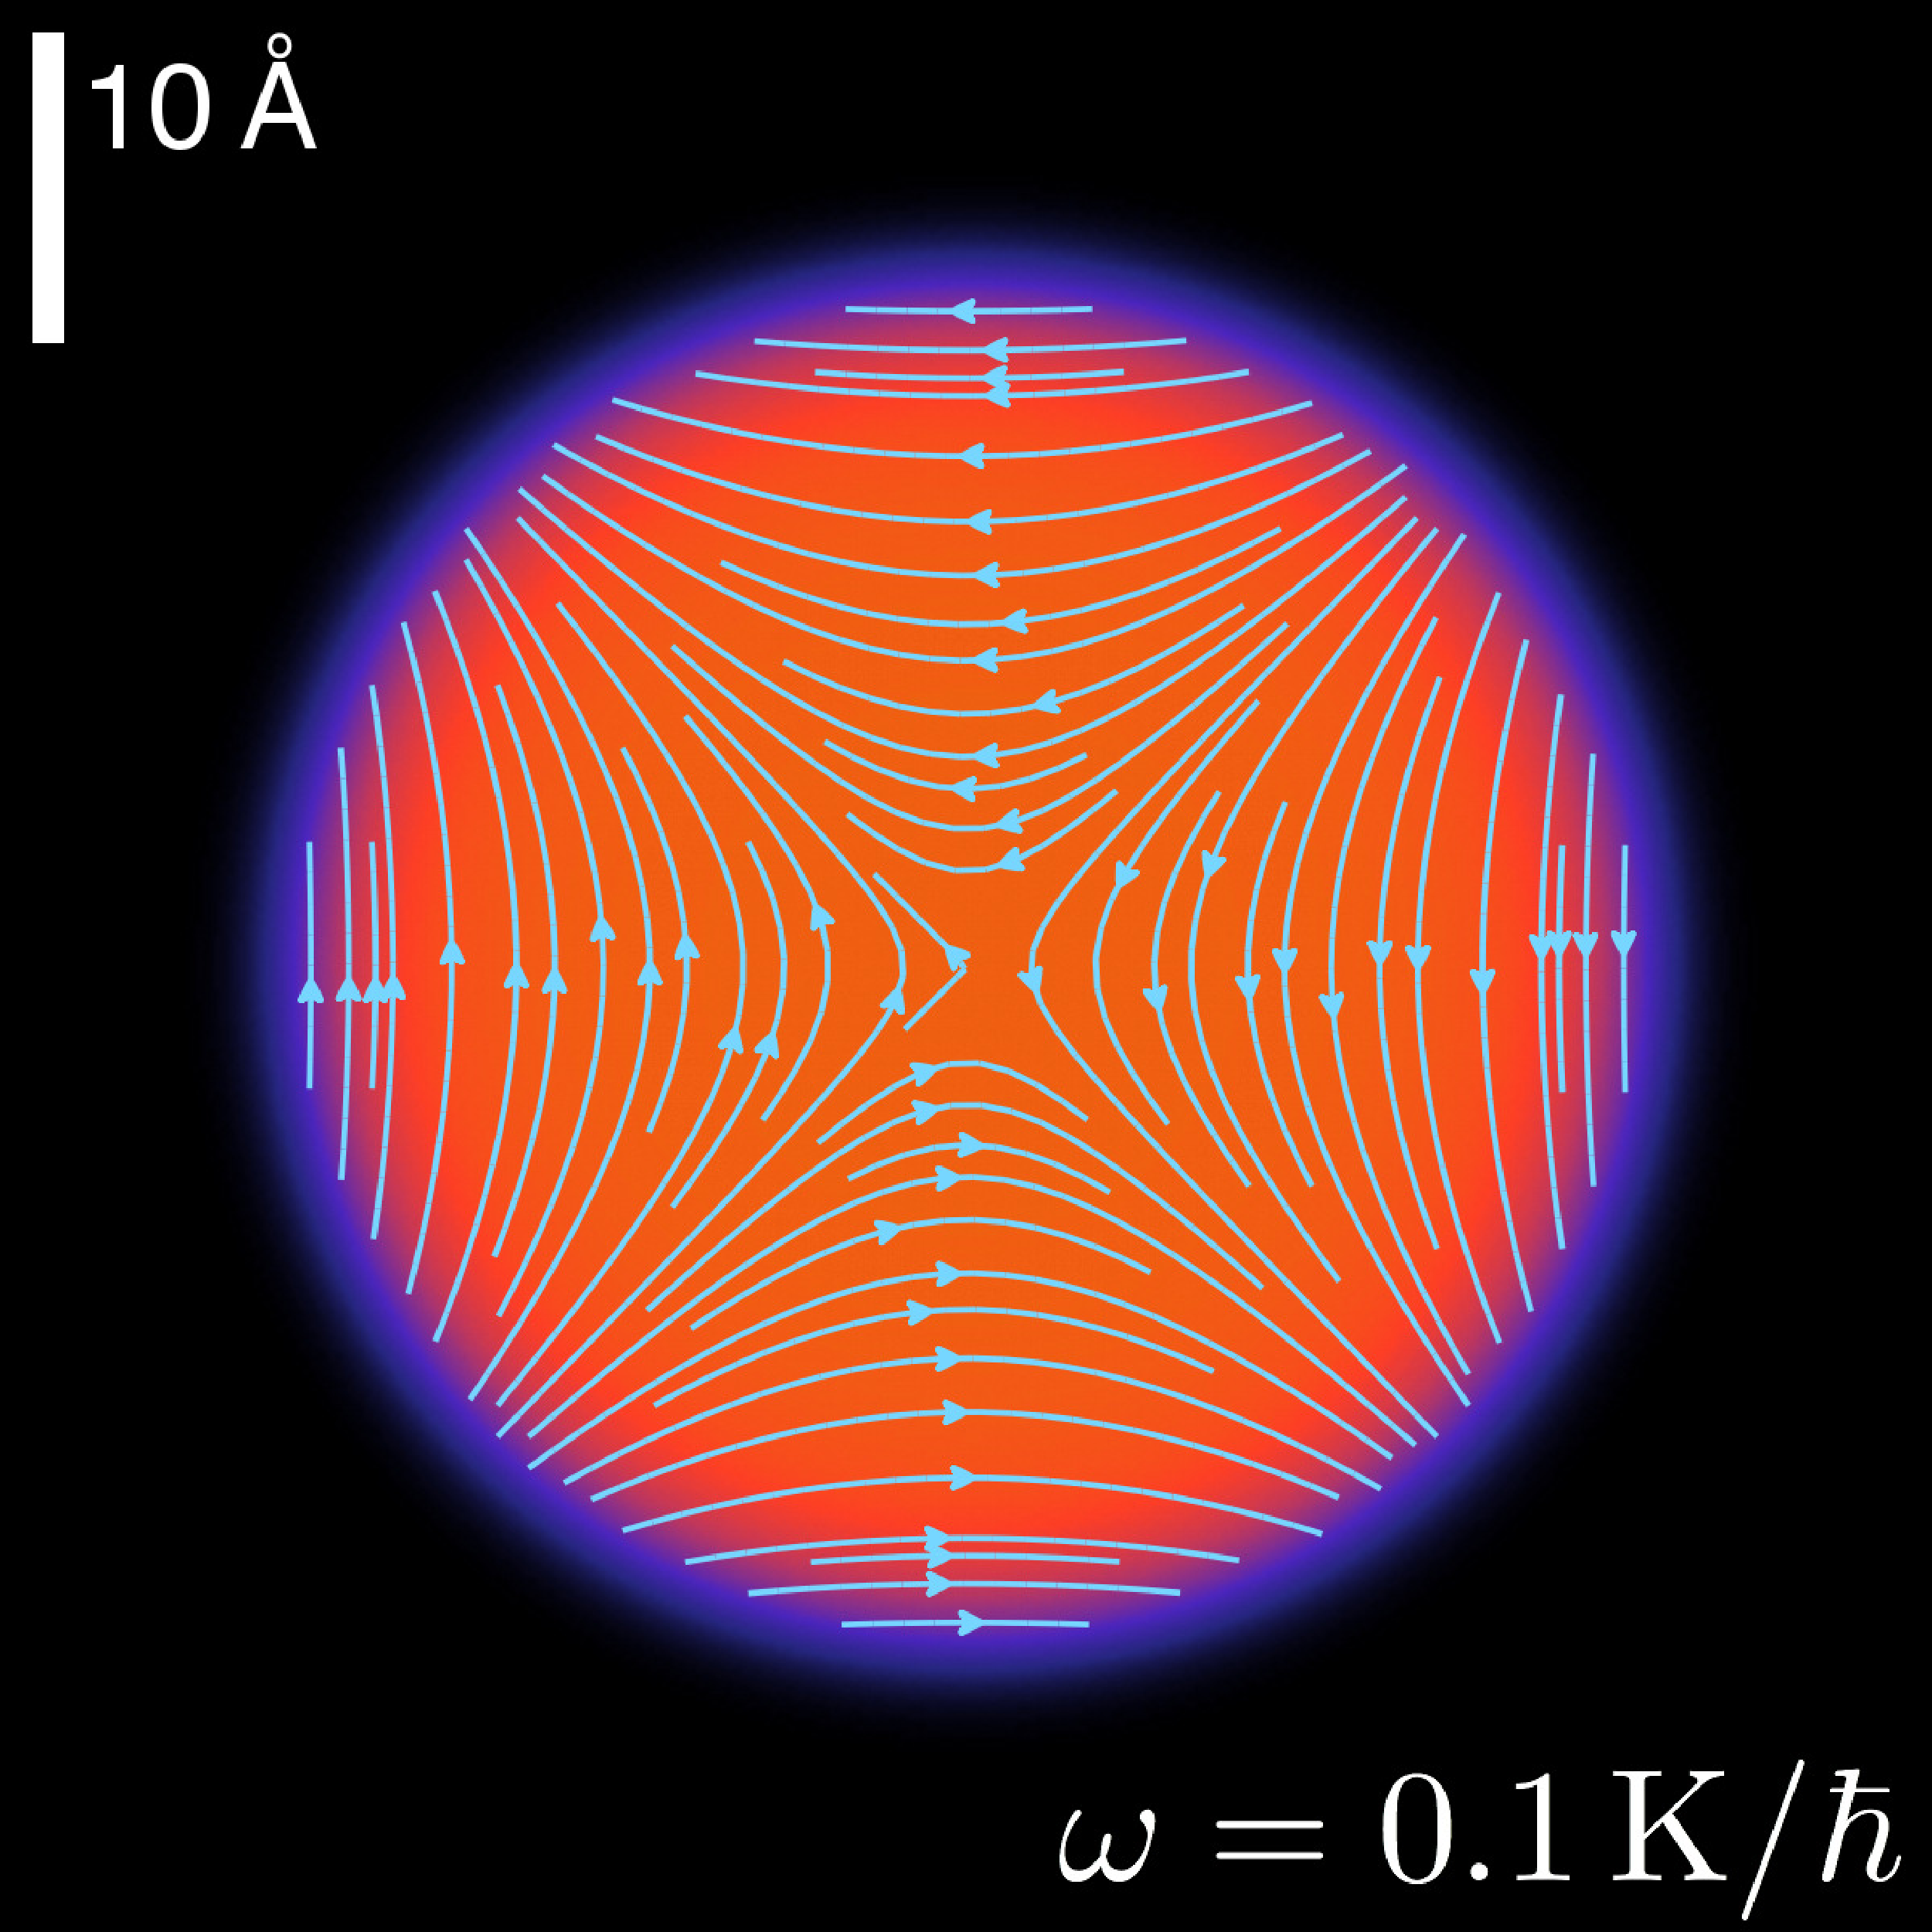
\includegraphics[width=0.7\linewidth,clip]{fig8}}
\caption{\label{fig8-capture} Stationary configuration of the $^4$He$_{1000}$ droplet at $\omega_c\gtrsim\omega=0.10\unit{K/\hbar}=0.0131\unit{ps}^{-1}$ in the corotating frame ($x-y$ plane). Superimposed is the irrotational velocity field arising from a velocity potential of the form $\mathcal{S}(\vec{r})=\alpha\,xy$.}
\end{figure}

%We have also looked at the appearance of vortex-antivortex (vortex dipole) configurations in the droplet. At variance with the two-vortex configuration, the 
%vortex dipole has zero angular momentum and  is stationary
%in the laboratory 
%frame.\citep{Fre10} We have obtained it by the imprinting procedure, giving to the vortex and  antivortex a different sign in the phase
% in Eq. (\ref{eq16}). Since this state has the same angular momentum as the vortex-free ground state of the droplet, we have implemented a Gram-Schmidt 
%orthogonalization procedure to obtain it. Figure \ref{fig9-capture} shows the resulting $^4$He$_{1000}$ droplet vortex dipole configuration. As compared to the two-vortex
%configuration, the droplet is less squeezed and deformed  due to its zero angular momentum.

%\begin{figure}[h]
%\centerline{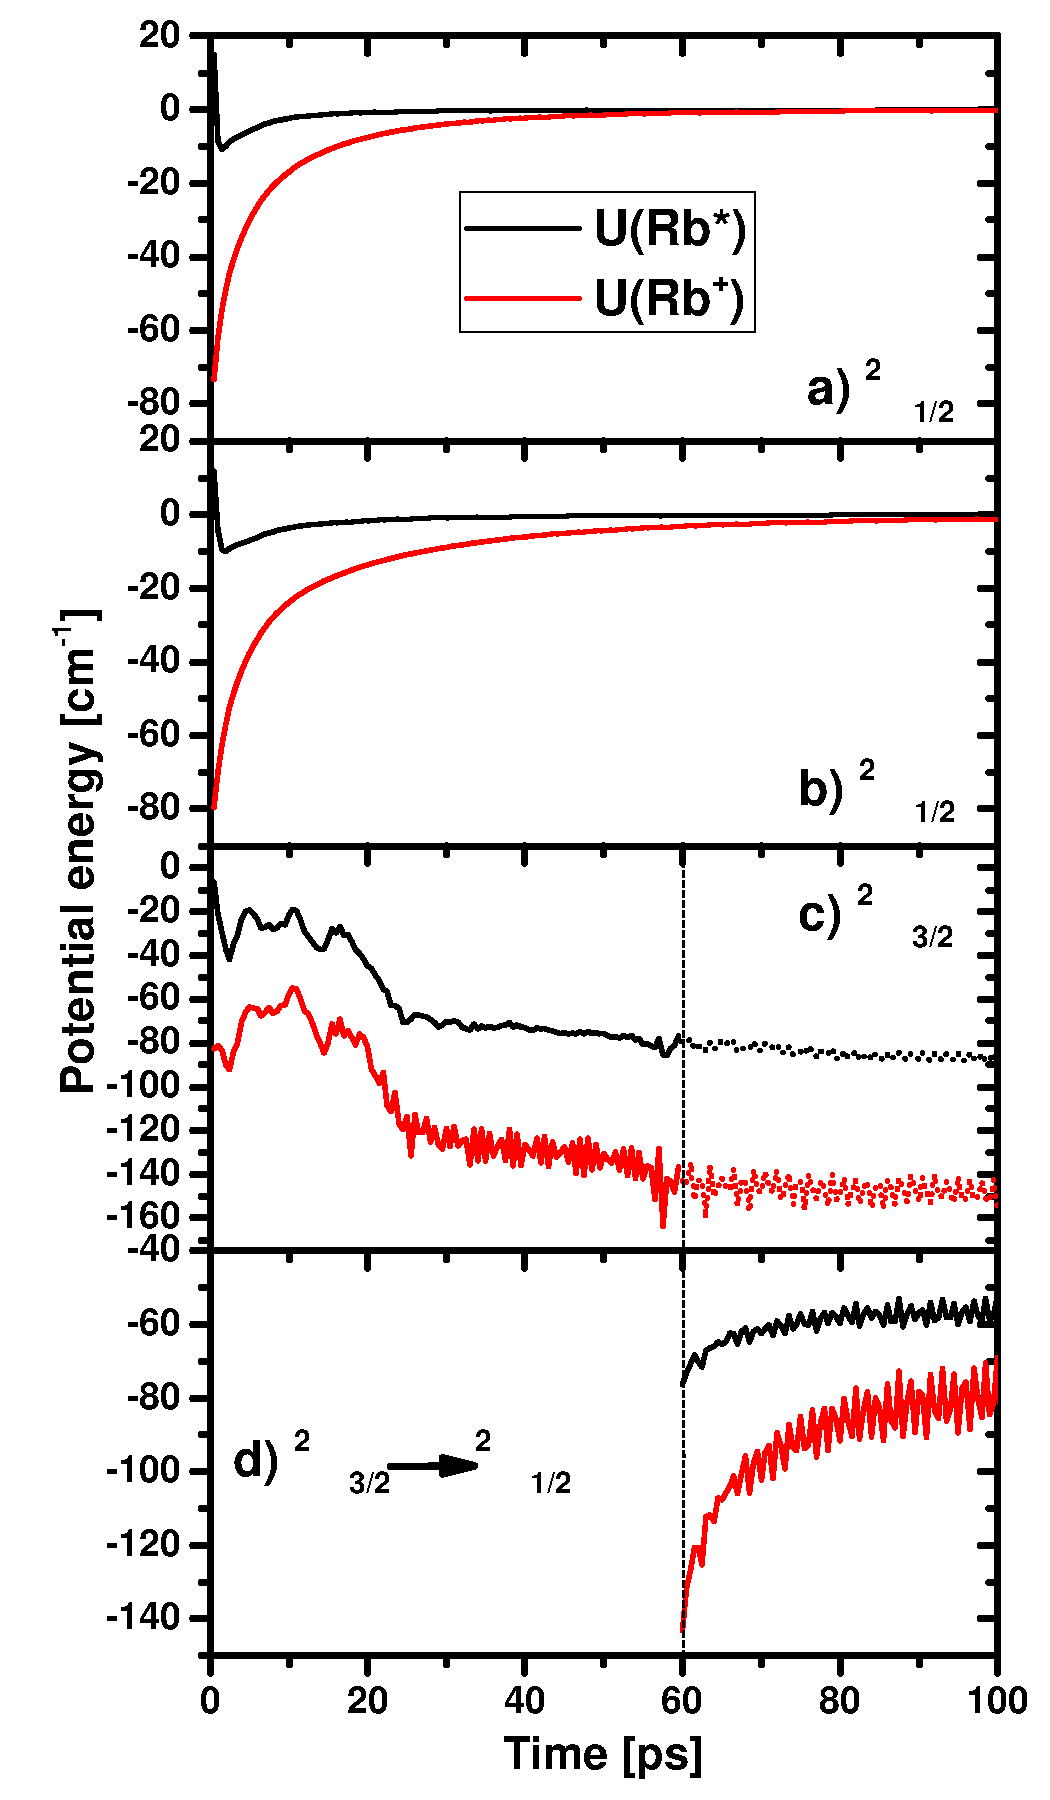
\includegraphics[width=0.9\linewidth,clip]{fig9}}
%\caption{\label{fig9-capture}
%$^4$He$_{1000}$ droplet vortex dipole configuration.  
%The left panel displays the helium density in the $x-z$ plane, and the right panel in the $x-y$ plane. 
%}
%\end{figure}

\section{Dynamics of  Xe and Ar capture by vortex lines}
To study the interaction of an atomic impurity with vortices, 
we have imprinted a vortex line in the $^4$He$_{1000}$ droplet 
and prepared the Xe atom in different kinematic conditions. 

%In a first simulation we have initially placed
% the Xe atom  inside the droplet 10 \AA{} away
%from the vortex line,   sending it  head-on towards the vortex at a velocity of 10 m/s.\citep{Coppens2017-2}
%This velocity  is of the order of the thermal velocity of a Xe atom in a droplet under experimental conditions,
%once the droplet has thermalized after capturing the Xe atoms  ($T \sim$0.4 K).\citep{Toe04}  
%Since the equilibrium position of  the Xe atom is at the center of the droplet, it  moves to this region and remains there during the rest of the simulation.
%In this region of the droplet, the Xe atom is also attracted by the vortex, but it is deflected by the superfluid flow around the vortex line and ends up orbiting around it. 
%Hence it is captured by the vortex without getting into its  core.
%The motion of the  atom
%produces sound waves in the liquid and distortions along of the vortex line (Kelvin modes) that will be shown in detail later.

%The kinematic conditions in the above simulation are similar  to those used for the simulation of inelastic scattering of xenon atoms by quantized vortices in superfluid bulk helium.\citep{Psh16}
% It has been  found in \citep{Psh16} that  a head-on collision leads to the capture of Xe by the vortex line for $v_0=$ 15.4 m/s , but not  for $v_0$=23.7 m/s.
%A detailed  analysis of the Xe capture as a function of the impact parameter has also been  carried out, with the conclusion that when the impact parameter 
% of the Xe atom approaching the vortex line is larger than about 5 \AA{}, Xe is deflected but not captured. In the case of droplets, the final result is very different.
%Upon capture the Xe atom wanders erratically inside the droplet,  as we have seen in the case of vortex-free droplets.
% The surface of the droplet deforms dynamically and acts as
% a ``pinball machine'',  which  eventually brings the Xe atom close enough to the vortex line if it missed it
% in the first attempt and was not previously ejected off the droplet. 
 
 The inelastic scattering of xenon atoms by quantized vortices in superfluid bulk helium has been addressed in\rf{Psh16}.
  It was found that
  a head-on collision leads to the capture of Xe by the vortex line for $v_0=$ 15.4 m/s, but not  for $v_0$=23.7 m/s.
We have carried out  an equivalent  simulation by initially placing
 the Xe atom  inside the droplet 10 \AA{} away
from the vortex line and   sending it  head-on towards the vortex at a velocity of 10 m/s.
This velocity  is of the order of the thermal velocity of a Xe atom in a droplet under experimental conditions,
once the droplet has thermalized after capturing the Xe atom  ($T \sim$0.4 K)\citep{Toe04}. 
Since the equilibrium position of  the Xe atom is at the center of the droplet, it  moves to this region and remains there during the rest of the simulation.
In this region of the droplet, the Xe atom is also attracted by the vortex, but it is deflected by the superfluid flow around the vortex line and ends up orbiting around it.
 Hence it is captured by the vortex without getting into its  core.

A detailed  analysis of the Xe capture as a function of the impact parameter has also been  carried out in\rf{Psh16}, with the conclusion that when the impact parameter 
 of the Xe atom approaching the vortex line is larger than about 5 \AA{}, Xe is deflected but not captured\citep{Psh16}.
  In the case of droplets, the final result is very different.
Upon capture, the Xe atom wanders erratically inside the droplet,  as we have seen in the case of vortex-free droplets.
 The surface of the droplet deforms dynamically and acts as
 a ``pinball machine'',  which  eventually brings the Xe atom close enough to the vortex line if it missed it
 in the first attempt or was not previously ejected off the droplet. 

%A more violent event takes place when the Xe atom is initially placed at rest on the droplet surface. This is the smoothest capture process one might think of, as no kinetic energy is 
%initially given to the impurity. The Xe atom is accelerated  towards the center of the droplet due to the attractive He-Xe interaction. 
%We show\citep{Coppens2017-2}  that, under these kinematic conditions, some He atoms are first drawn towards the  impurity because they are lighter, see also Figs. \ref{fig10-capture} and \ref{fig11-capture}. 
%A similar effect was found in the sinking of Cs$^+$ and Rb$^+$ cations.\citep{Lea14b} 
%Eventually, the impurity with its ``solvation structure'' sinks, acquires some velocity, and is also deflected by the velocity field of the 
%vortex line. 


%A more violent event takes place when. 
The smoothest capture process one might think of corresponds to  the Xe atom being initially placed at rest on the droplet surface, as no kinetic energy is 
given to the impurity. The Xe atom is accelerated  towards the center of the droplet due to the attractive He-Xe interaction. 
We show  that, under these kinematic conditions, some He atoms are first drawn towards the impurity because they are lighter, see also \fig{fig10-capture}, \fig{fig11-capture} and the Electronic Supplementary Information available at doi: \href{http://dx.doi.org/10.1039/C7CP03307A}{10.1039/C7CP03307A} for the continuous movie corresponding to the simulation. 
%A similar effect was found in the sinking of Cs$^+$ and Rb$^+$ cations.\citep{Lea14b} 
Eventually, the impurity with its ``solvation structure'' sinks, acquires some velocity, and is also deflected by the velocity field of the 
vortex line. 

 We have tried two different initial locations of the Xe atom on the droplet surface.  One is  a point on the equator of the droplet, in a plane perpendicular to the vortex line; 
 the other location is one of the open vortex core ends.  Our aim was to see if a sensible difference in the transit time of Xe across the droplet
could be detected.  The simulations do not show important differences between the time taken by the impurity to reach the center of the droplet. It is about 20~\% larger
when Xe starts from the equator than from the core end\citep{Coppens2017-2}. It is worth noting that  in the latter case the sliding of the impurity along the core proceeds rather smoothly, and that the impurity
oscillates back and forth much as in the vortex-free case. 

The simulation of Xe ($v_0$=200 m/s) and Ar ($v_0$=360 m/s) atoms head-on colliding with a $^4$He$_{1000}$ droplet perpendicularly to the vortex line has been analyzed and
compared with the result corresponding to a vortex-free droplet. The trajectory of the Xe and Ar atoms in phase space is shown \fig{fig3-capture}. In both cases the trajectory of the impurity
is limited to the region of the droplet around the vortex line. The impurity orbits around the vortex line because the superfluid flow does so. Since in the DFT approach
no dissipation is included, the signature of the capture of an impurity by a vortex is its close orbiting around the vortex line, as shown in the figure
and especially in\rf{Coppens2017-2}. The ESI material shows that whereas Ar is captured during its first transit across the droplet, the Xe atom is only captured in its second transit. We attribute this difference 
to the larger solvation energy of Xe (see \scn{sec:vtx-lines}), which requires more time to be dissipated. It can be seen\citep{Coppens2017-2} that when Xe detaches from the vortex  in the first
transit,   the  vortex line is reconnected near the atomic solvation structure because no open ends can remain in the bulk of the droplet.
  
%As found in previous simulations,\citep{Lea16,Cop16} 
\fig{fig10-capture} and \fig{fig11-capture} show that
 when the impurity hits the droplet surface a series of surface and volume density waves are launched.
These waves travel  much faster than the impurity itself, 
which has lost a large amount of kinetic energy when it pierced the surface.

The displacement of the  atom in the droplet
produces sound waves in the liquid and distortions along the vortex line (Kelvin modes). 
It is worth seeing that before the bending by the collision with the impurity, the vortex line is twisted (helical Kelvin mode). 
  This  is due to the interference between the  spherical wave front flow
 produced by the hitting of the droplet surface, that travels from bottom to top, 
 and the  flow around the vortex core.
 The spherical wave front  hits first the central portion of the vortex line, whose ends are anchored on the droplet surface. This yields the appearance of the helical distortion
 along the vortex line shown in \fig{fig12-capture}.
 The twisting  can no longer  be followed after the
 impurity solvation structure reaches the vortex line, bending and dragging it along in the course of its orbiting around it. But it is clearly visible before as shown in \fig{fig12-capture}, that displays the
 density of the droplet around the vortex line at the indicated collision time. 

\begin{figure}[h]
\centerline{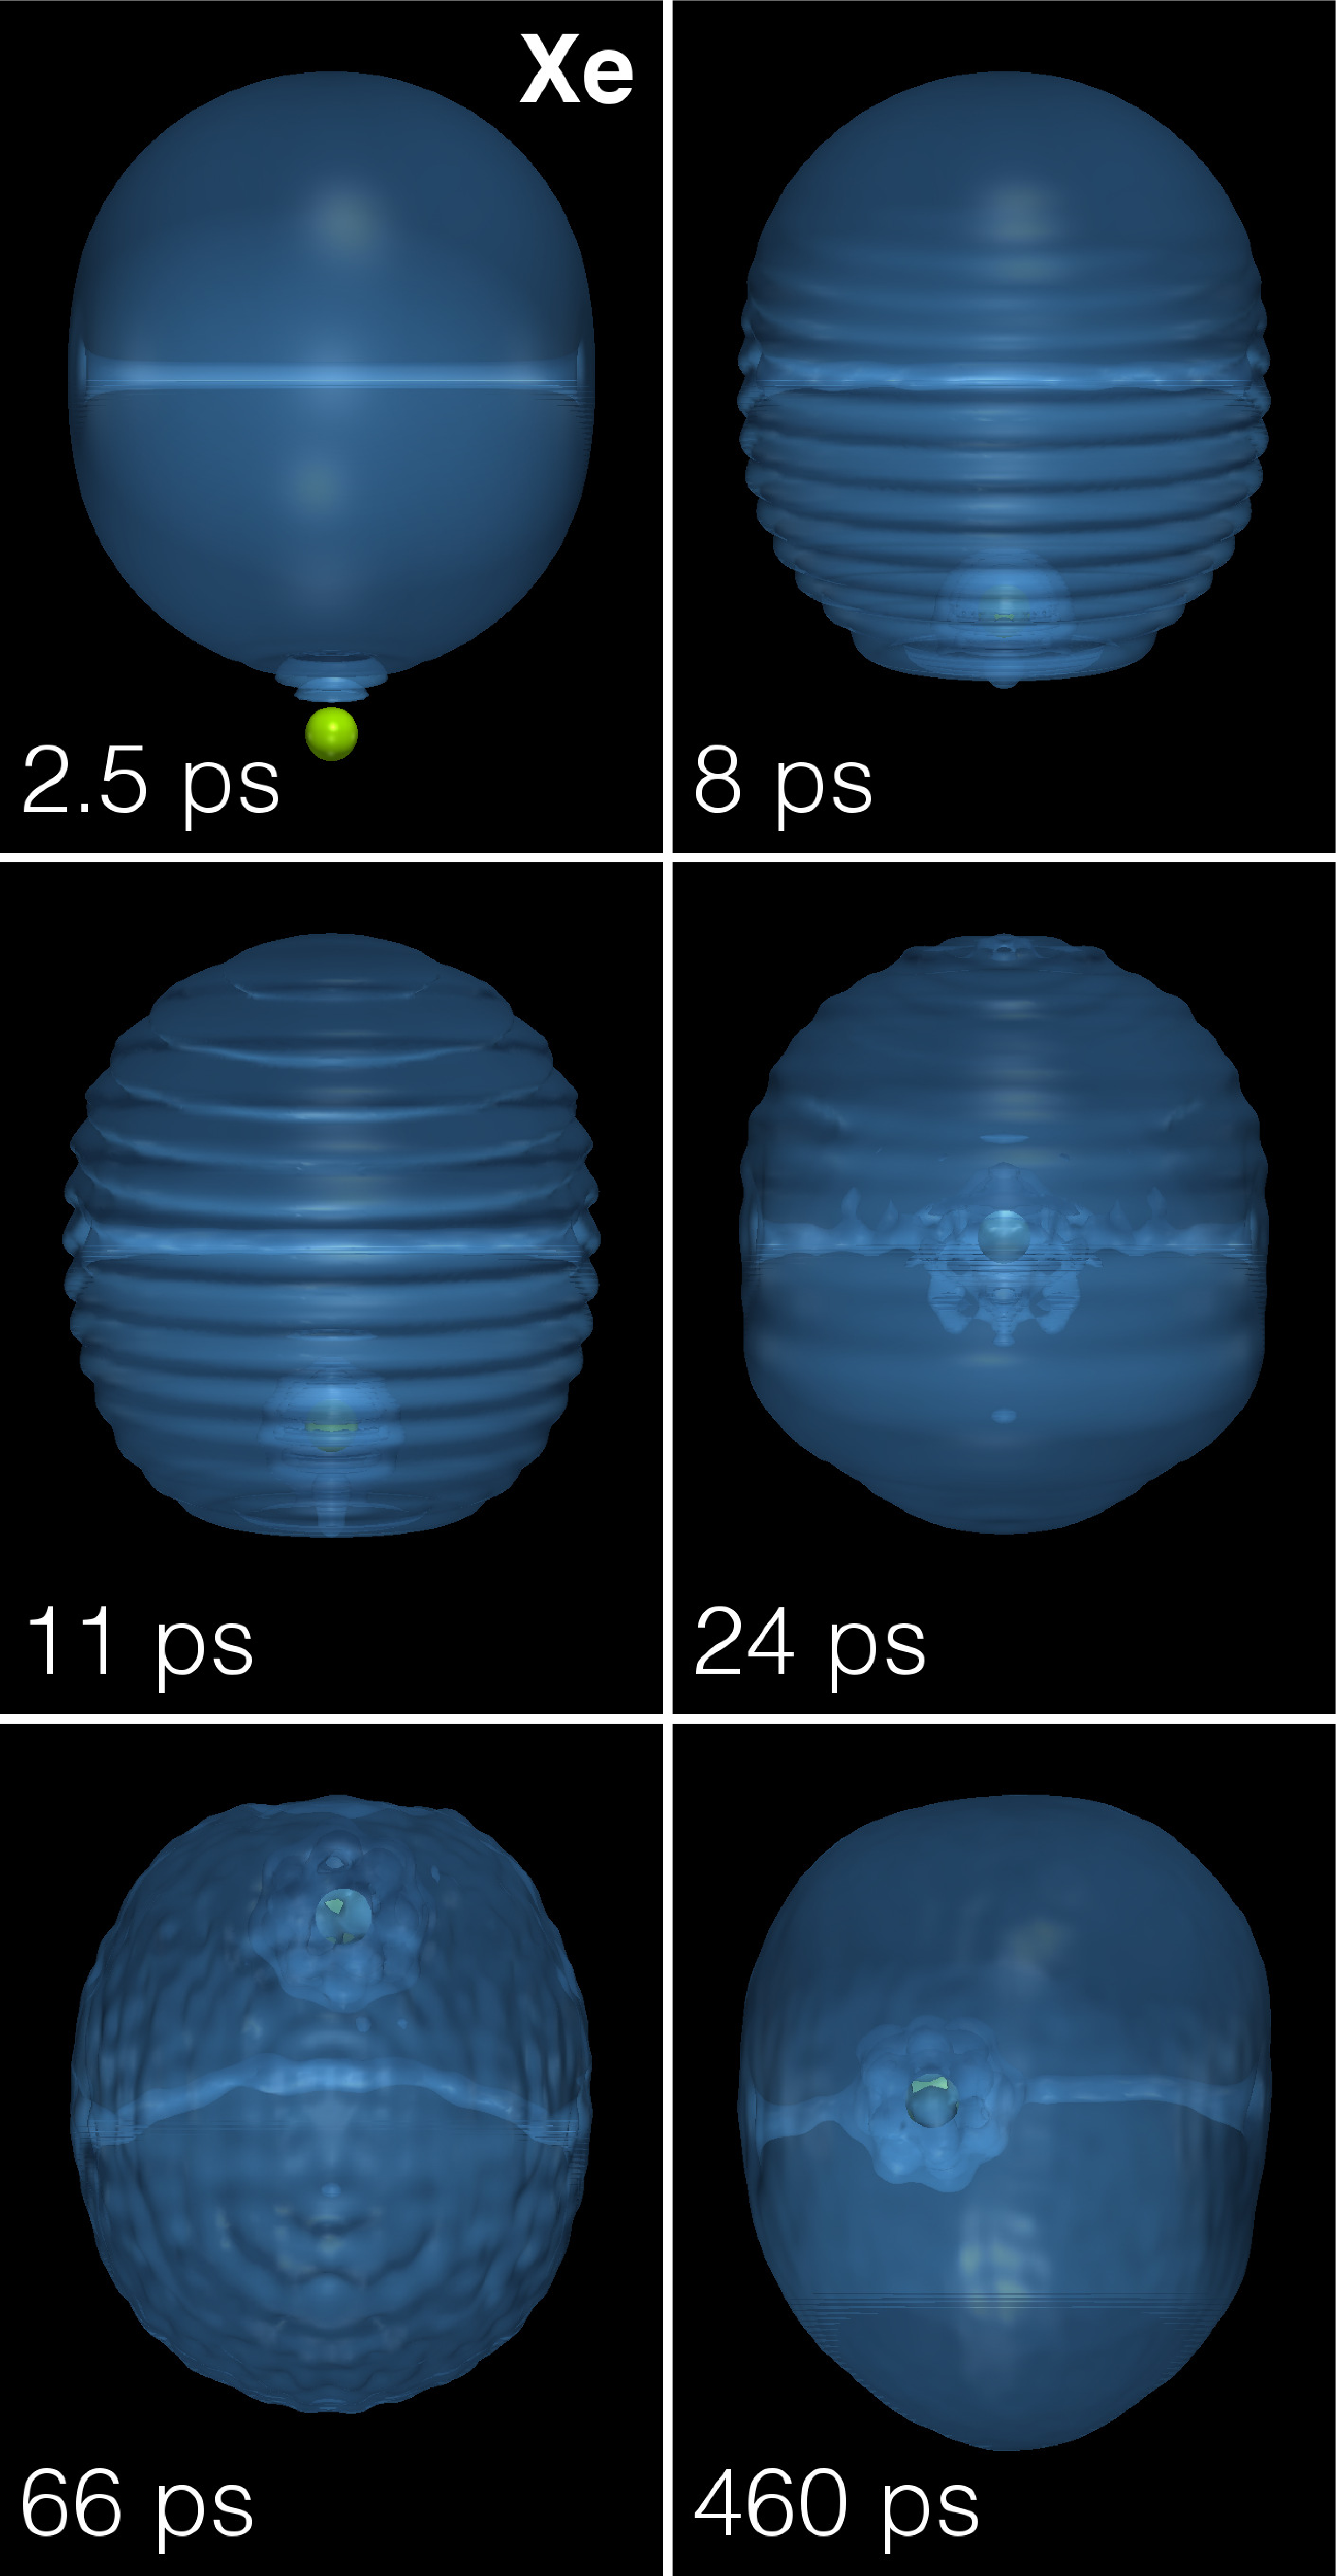
\includegraphics[width=0.60\linewidth,clip]{fig10}}
\caption{\label{fig10-capture}
Dynamic evolution of a Xe atom (green dot) approaching a $^4$He$_{1000}$ 
droplet  hosting a vortex line from below at $v_0 = 200$ m/s. The corresponding time is indicated in each frame\citep{Coppens2017-2}.  
}
\end{figure}


\begin{figure}[h]
\centerline{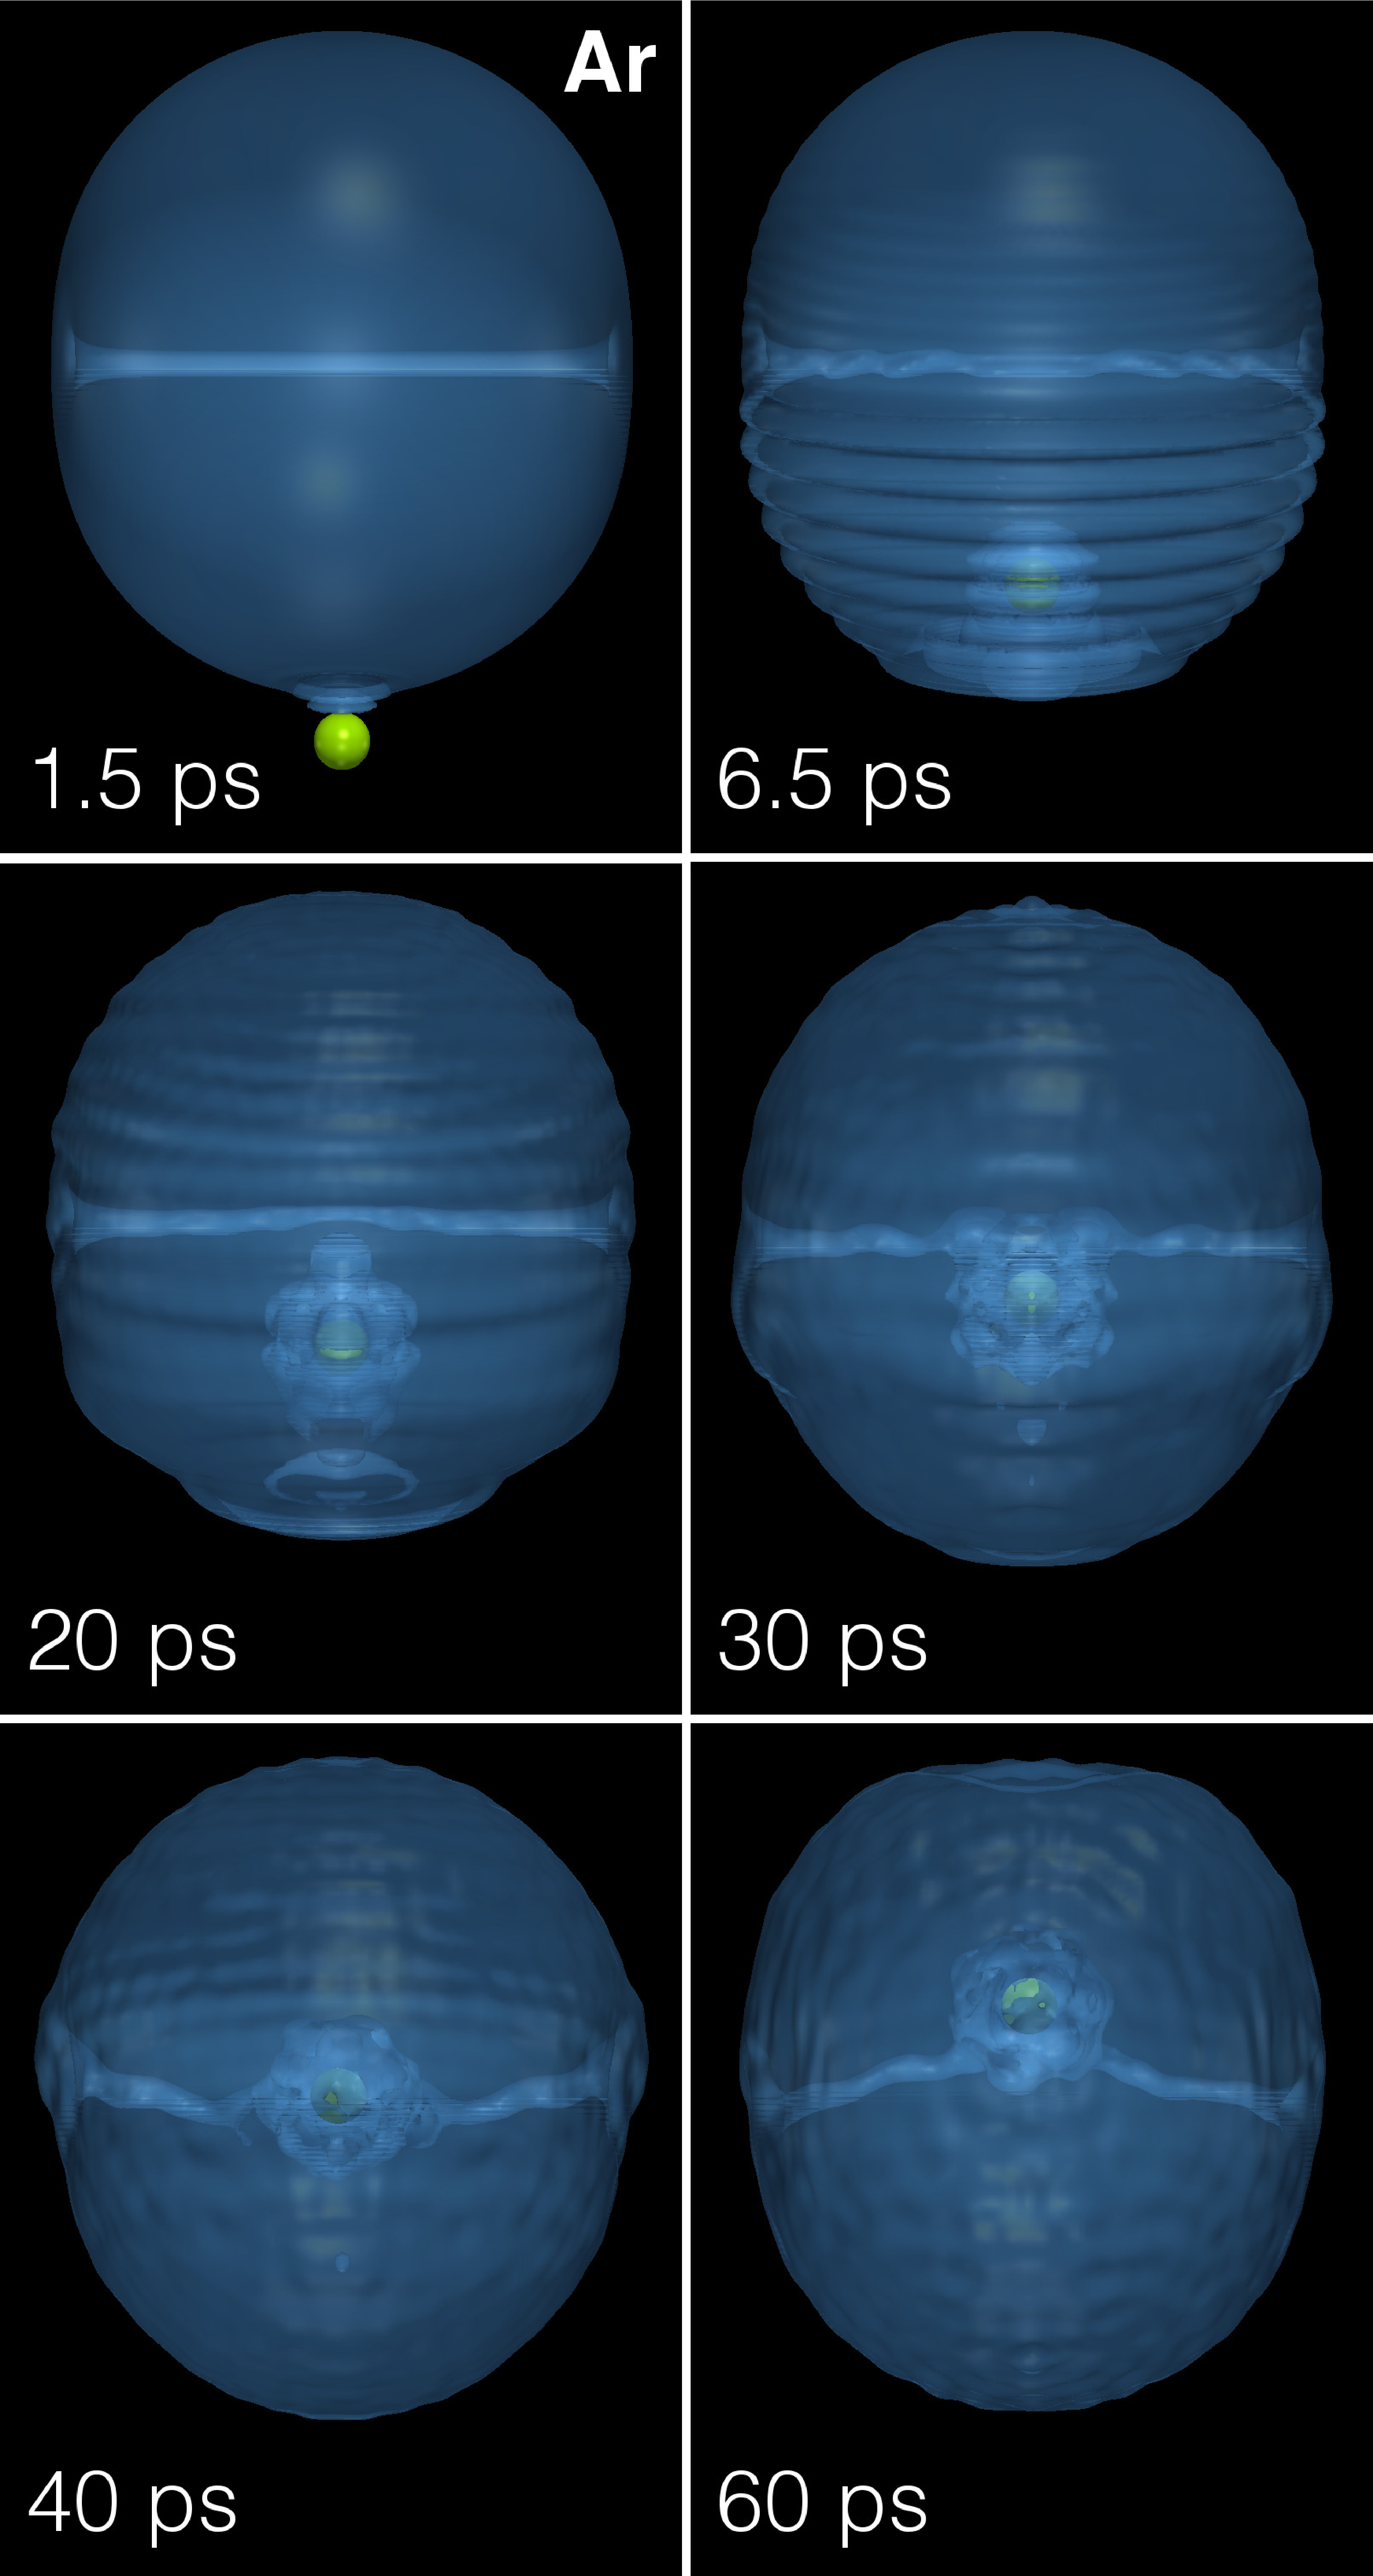
\includegraphics[width=0.60\linewidth,clip]{fig11}}
\caption{\label{fig11-capture} 
Same as \fig{fig10-capture} for an Ar atom at $v_0 = 360$ m/s\citep{Coppens2017-2}.
}
\end{figure}

 
% Finally, we have simulated the 
%collision of a Xe  atom at 200 m/s against a $^4$He$_{1000}$ droplet hosting a vortex dipole.
%As shown in the  ESI$\dag$ material,\citep{Coppens2017-2} the Xe atom attaches to either of the vortex cores in the course of the dynamics. After several hundred ps we have 
%found that the impurity eventually gets stuck  to one of the vortices of the dipole and not to both simultaneously. 
%We attribute this to the large superfluid flow in the region between
%them. The situation might change 
%for a configuration made of two vortices with the same sign,
%where superfluid flows tend to cancel out in that region. We have not explored this possibility.   

We have thus shown that   Xe and Ar atoms are readily captured by vortex lines in helium droplets under conditions prevailing in the experiments\citep{Gom14,Jones2016}. Simulating the 
capture of a huge number of  impurities or clusters by vortex arrays in  very large droplets is beyond reach at present. However, the results presented in
this subsection are the proof of concept that the limitation is technical and not conceptual.

\begin{figure}[h]
\centerline{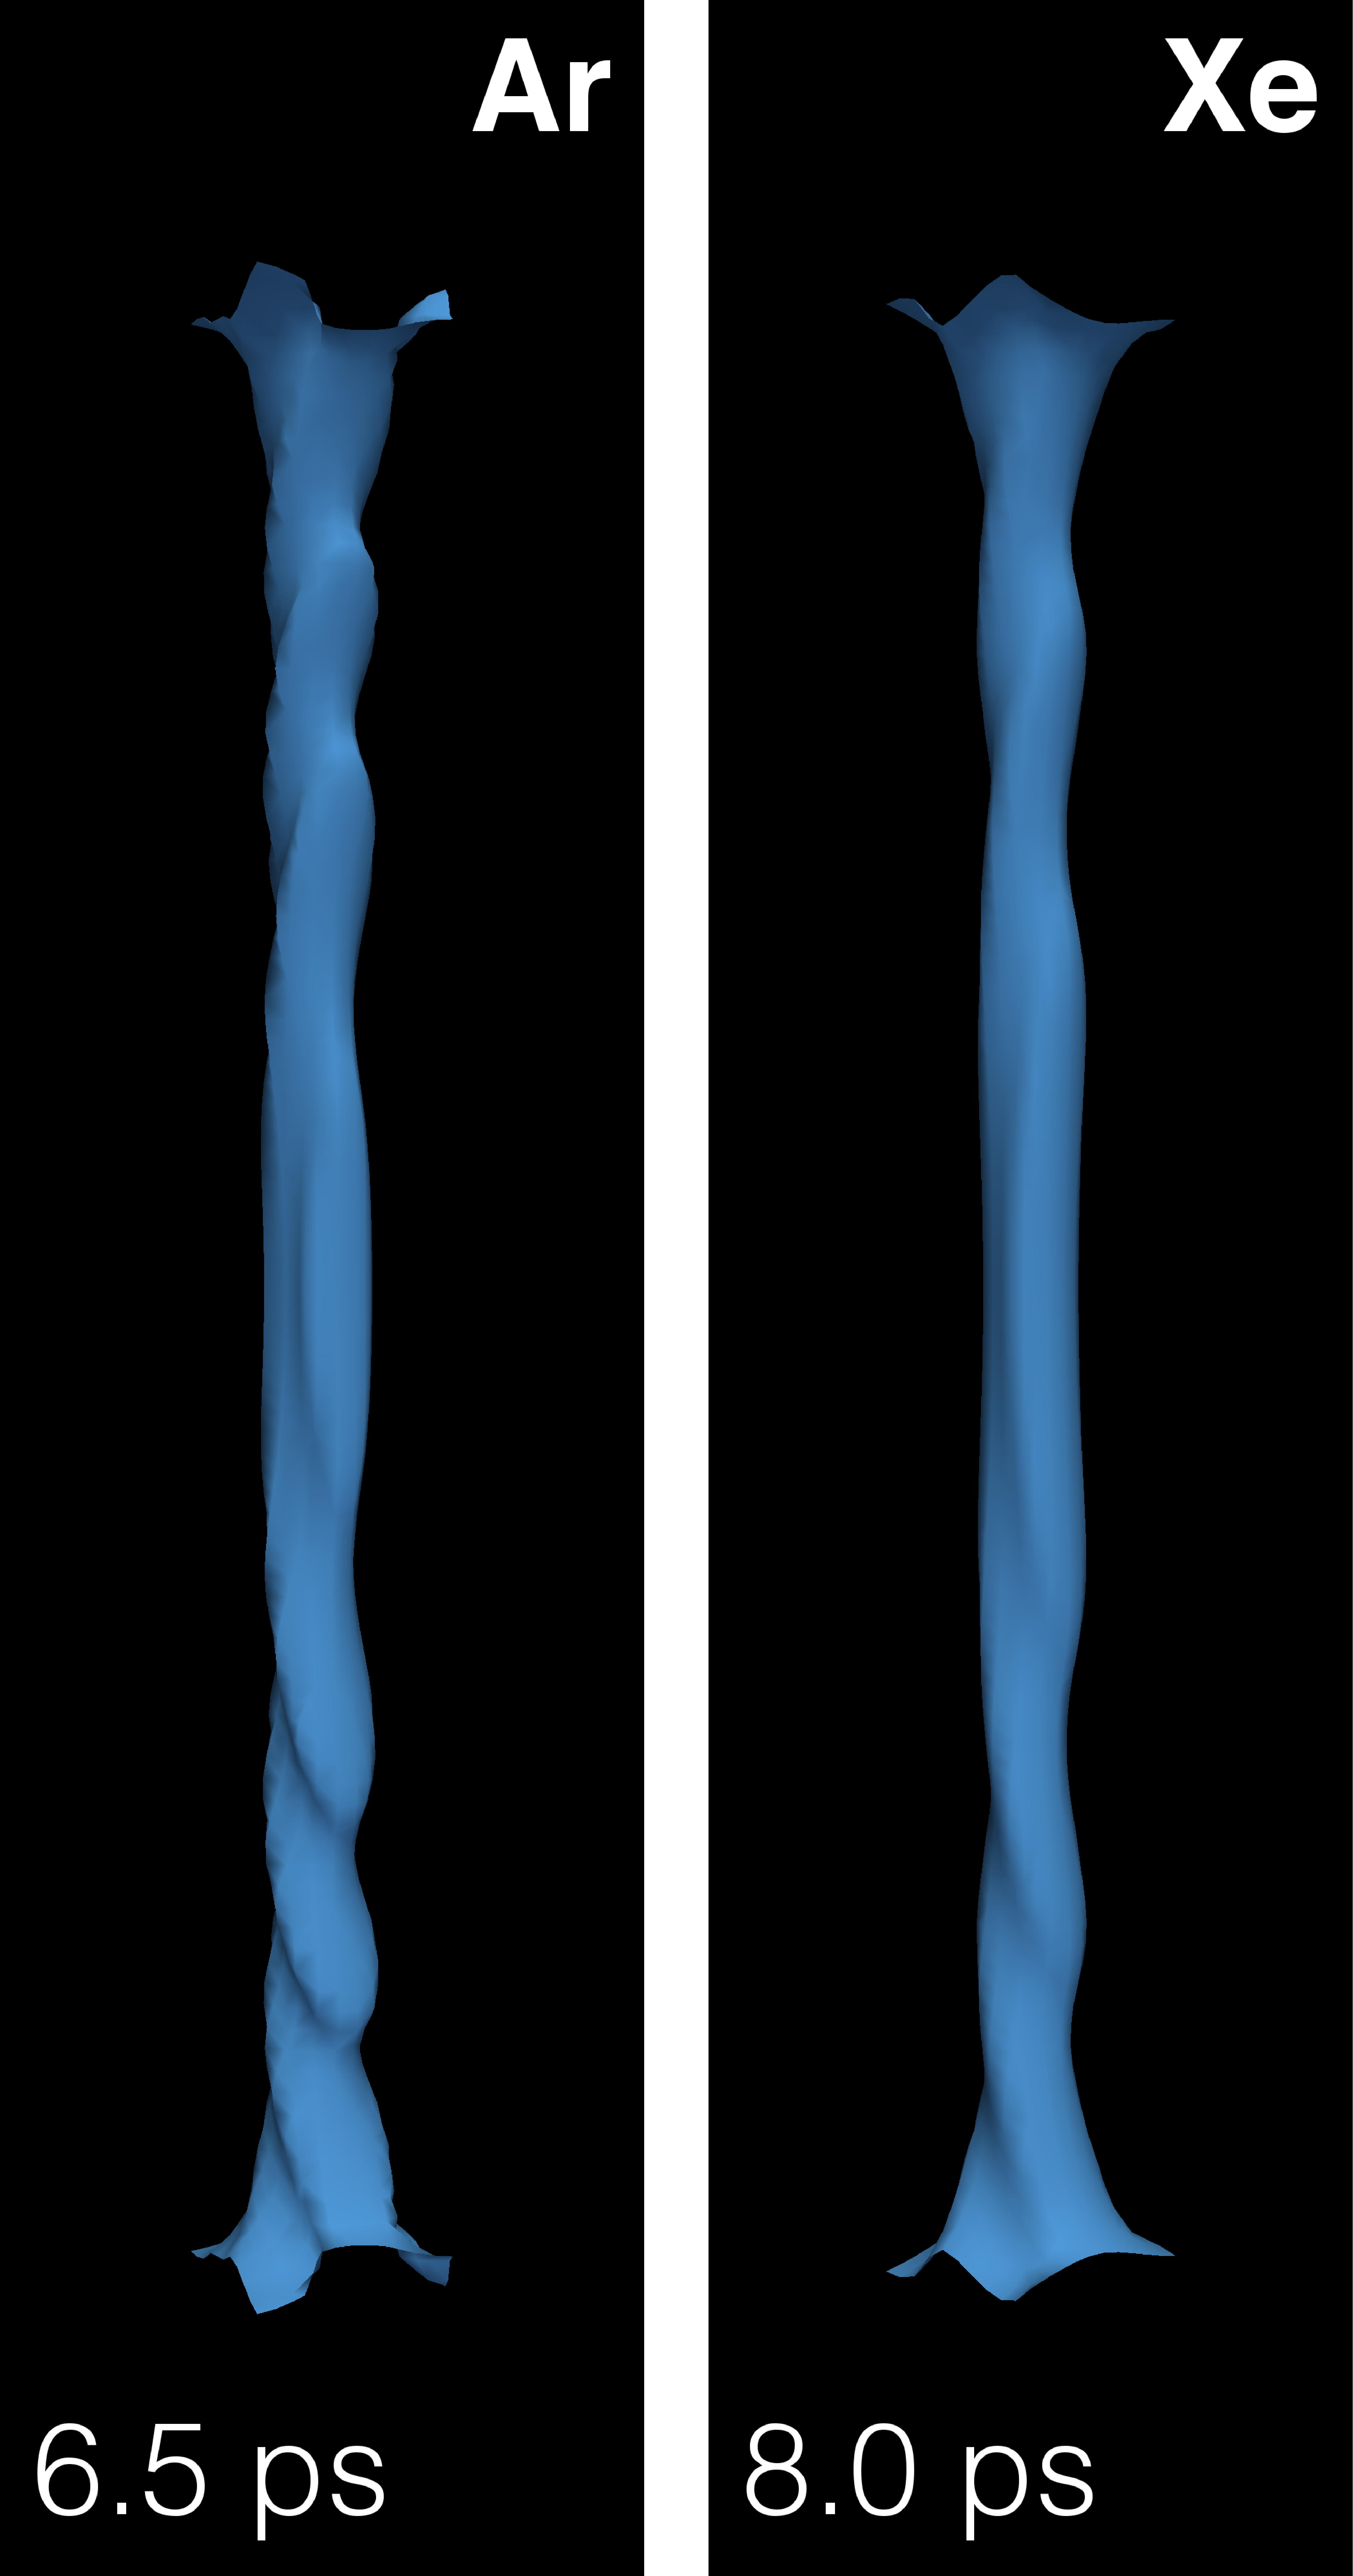
\includegraphics[width=0.60\linewidth,clip]{fig12}}
\caption{\label{fig12-capture} 
Core structure of the vortex line in a $^4$He$_{1000}$ droplet after colliding  with  Xe at $v_0$=200 m/s (right panel, $t= 8$ ps) and Ar at 360 m/s (left panel, $t$=6.5 ps). 
The  full structure of the droplet is shown in \fig{fig10-capture} and \fig{fig11-capture}.
}
\end{figure}
  
\section{Vortex arrays in $^4$He droplets doped with Ar atoms}

The existence of ordered vortex lattices inside $^4$He droplets has been established  by the appearance of Bragg patterns from 
Xe clusters trapped inside the vortex cores  in droplets made of $N= 10^8 - 10^{11}$ atoms
(corresponding to radii from 100 to 1000 nm)\citep{Gom14,Jones2016}. We have 
recently studied the stability of vortex 
arrays made of up to $n_v=9$ vortices
inside a $^4$He nanodroplet using the DFT approach\citep{Anc15}.  
It was found that 
the energetically favored structure for $n_v > 6$ is a ring 
of vortices encircling a vortex at the center of the droplet.
Fot $n_v=6$,  the 
configuration with a six-vortex ring is found to have almost 
the same energy as the five-fold ring
plus a vortex at the center. The former structure 
has been experimentally observed\citep{Gom14,Jones2016,Ber17}, 
although classical vortex theory 
predicts for it a much higher free energy cost than for the latter\citep{Cam79}.
Similar equilibrium structures have been obtained within DFT for
helium nanocylinders hosting vortex arrays\citep{Anc14}.

In the experiments of\rf{Jones2016} the diffraction images 
show that rotating $^4$He nanodroplets of about 200 nm in diameter 
contain a small number of symmetrically arranged quantum 
vortices whose cores are filled with regularly spaced 
Xe clusters. Unexpected large distances 
of the vortices from the droplet center ($\sim 0.7-0.8$ droplet radii) 
are observed and explained as a result of the balance between 
the contribution of the Xe atoms to the total angular momentum of the droplets and 
the solvation potential of the embedded Xe atoms, which opposes the migration of vortices
towards the droplet surface and their annihilation there, as it would
happen instead in the case of undoped vortices for low values of the
droplet rotational frequency.

\begin{figure}[!]
\centerline{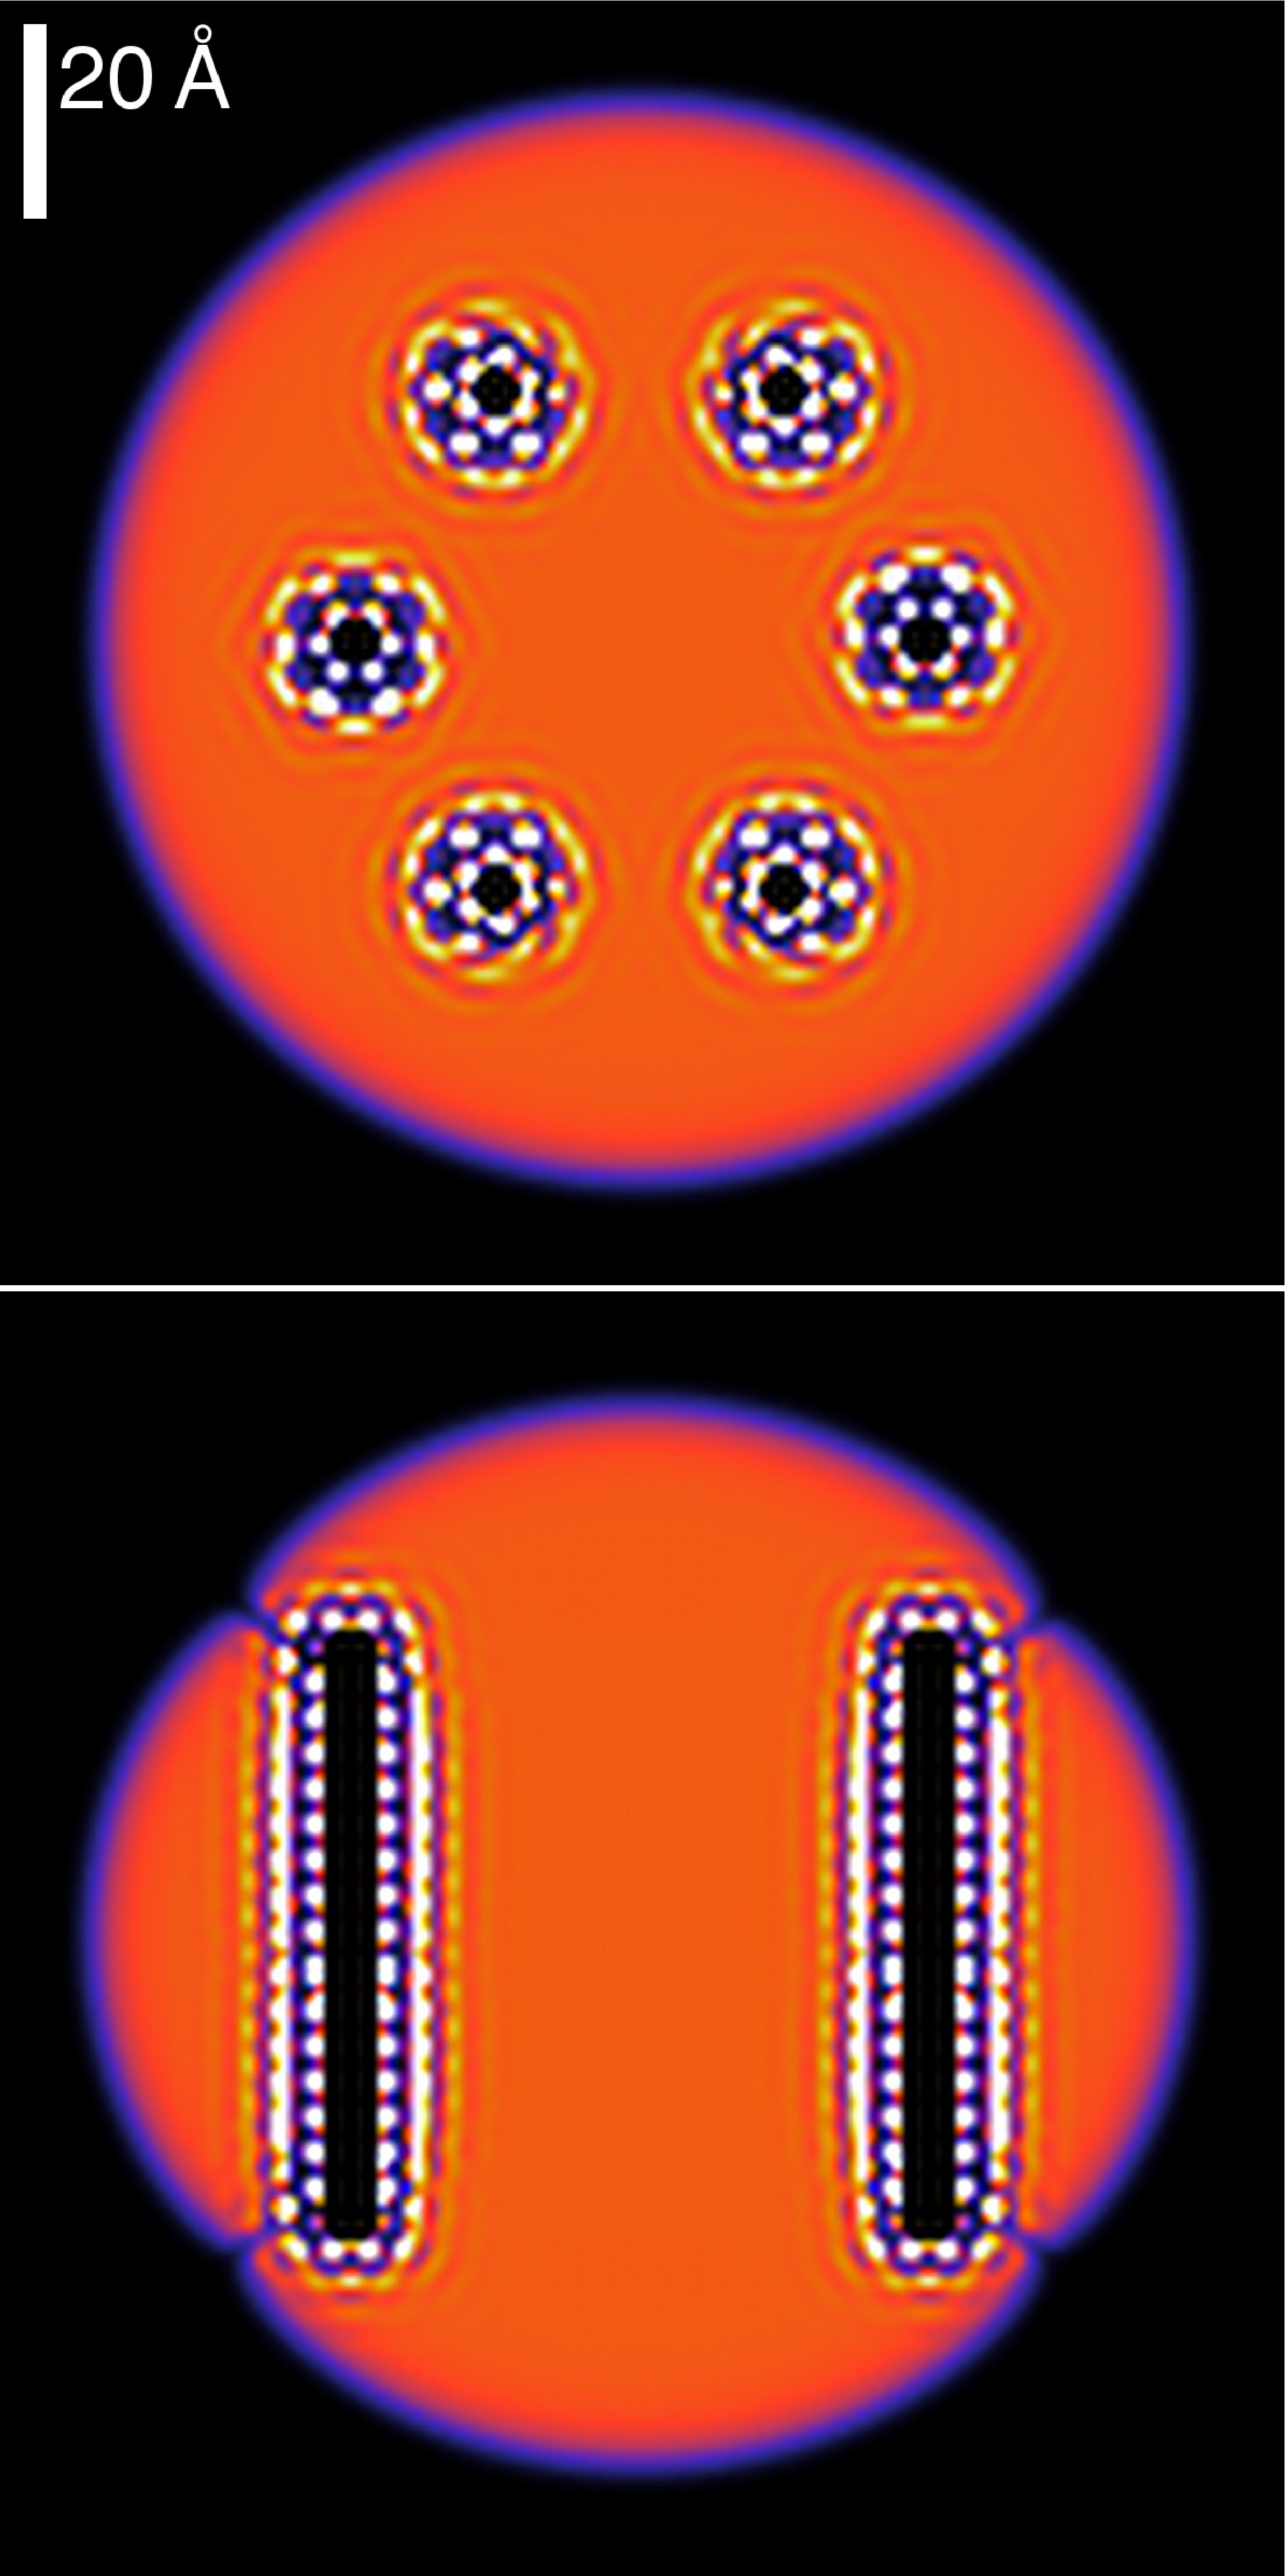
\includegraphics[width=0.6\linewidth,clip]{fig13}}
\caption{\label{fig13-capture} 
Helium droplet configuration hosting six vortices, each doped with a line of 
regularly spaced Ar atoms (not represented). 
The top figure shows the density in the $x-y$
symmetry plane (top view), while the bottom figure shows a side view corresponding to the 
$y-z$ plane. 
As in some of the previous figures, the bright  spots are high density blobs appearing around the impurity atoms.
}
\end{figure}

\begin{figure}[!]
\centerline{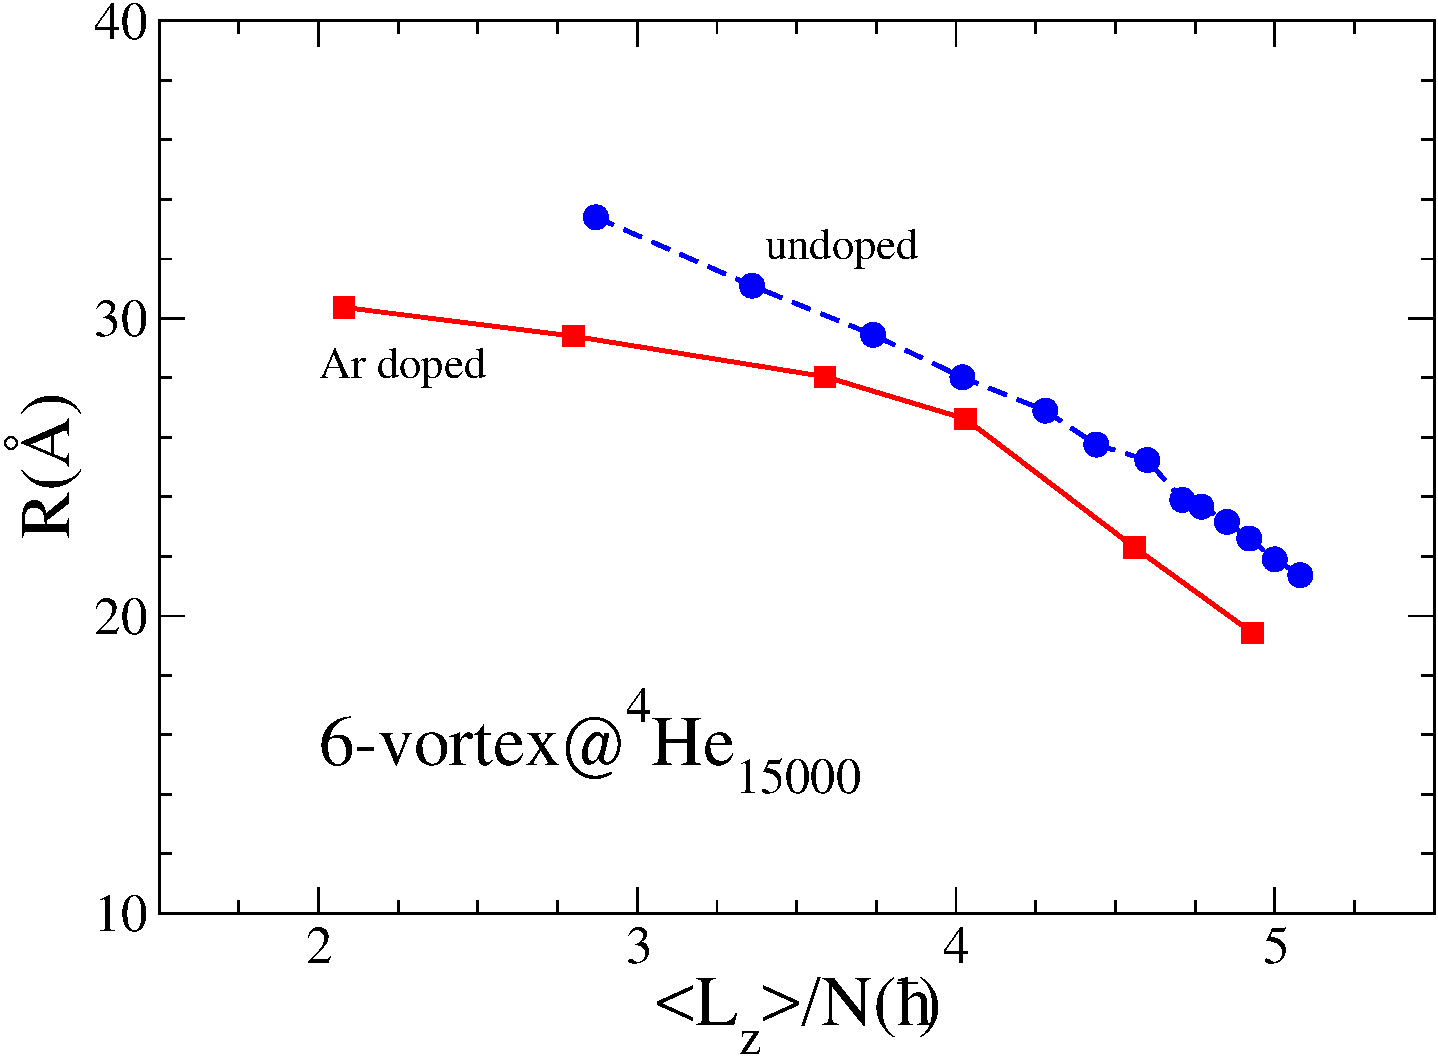
\includegraphics[width=0.9\linewidth,clip]{fig14}}
\caption{\label{fig14-capture} 
Calculated equilibrium distance of the 6-vortex ring
from the droplet center as a function of the 
angular momentum per He atom in units of $\hbar$. 
The dots represent the results for undoped vortices, while the squares are the results for 
Ar-doped vortices. The lines are drawn as a guide to the eye.
}
\end{figure}

In practice, as more and more Xe atoms become
attached to a vortex, they adopt the angular velocity of its
revolution about the droplet center. 
If the Xe capture is isotropic, the total angular momentum of the droplet is conserved, and 
thus the angular momentum accompanying the Xe rotational motion must be
transferred from the vortices to the impurities. This reduction in the angular momentum of the
vortices causes them to move outwards, 
resulting in the larger
equilibrium distances of the vortices observed in 
the experiments. The actual equilibrium radial positions
result from a balance between this tendency to 
move towards the droplet surface 
and the solvation potential, 
which tends instead to draw impurities towards the droplet
center.

We have looked for stationary configurations of a 6-vortex ring
in a rotating He$_{15000}$ droplet by solving the
EL equations in the corotating frame with a fixed
angular velocity. Each vortex core is filled with Ar
atoms, and the system is allowed to fully relax.
In the end, the column of atoms inside each vortex core reaches an equilibrium structure 
where the Ar atoms are separated by a distance which  is roughly that of the Ar dimer.
One such configuration is shown in \fig{fig13-capture}. Note that 
the vortex cores are almost straight lines, whereas in an
undoped droplet rotating with the same velocity 
the vortex lines would be bent, 
as shown  e.g. in \fig{fig7-capture}.
The Ar atoms are not shown in the Figure.
The localized structures appearing in the vortex cores are 
regions of highly inhomogeneous, high  $^4$He density
resulting from the Ar-He attractive potential.
% and \ref{fig9-capture}.

The presence of impurities thus confers rigidity to the vortex lines,
preventing them from bending. Yet, the small segment of the vortex line free from impurities bends so as to hit 
the droplet surface perpendicularly, see the bottom \fig{fig13-capture}.
Note that in the absence of vortices, Ar atoms initially placed
in a linear chain structure would relax towards the lower energy, compact 
configuration of an Ar cluster in the bulk of the droplet.
However, once trapped by a vortex core, their collapse 
into such a cluster structure does not occur,
i.e. an energy barrier appears and prevents the formation of Ar
clusters. 
%As commented below, 
Our simplified 
description of the more complex experimental 
conditions (where each vortex line hosts chains of regularly spaced
atomic clusters, instead of chains of single atoms)
is due to computational limitations.

Our choice of Ar instead of Xe as a dopant is motivated by the weaker He-Ar and Ar-Ar interactions, which 
facilitates the imaginary-time relaxation. The interaction of the helium environment with several close-by impurities increases the 
strength of  dopant-droplet interaction, producing  
helium localization around the impurities (snowball structures), see \fig{fig10-capture}. Stabilizing these
structures is extremely time consuming, 
especially when the He-impurity interaction is strong.
Experiments were also carried out with Ar atoms as dopants, 
but have not been analyzed yet\citep{note}.
However, no significant difference is expected between argon and xenon, 
neither from the experimental nor from the theoretical viewpoint.

There are obvious differences in scales between our simulations and  
 the actual experiments,  due to  computational 
cost. In experiments heavier impurities are used (Xe), 
the droplets are much larger
and the doping is known to occur by filling the vortex cores with a chain 
of equally spaced Xe clusters, each made of
hundreds of atoms, instead of atom chains as done in our simulations.
In spite of these differences, we find results which  
qualitatively explain the unusual behavior of vortex lines 
experimentally observed in doped rotating helium droplets.

We have looked for the equilibrium structure of the Ar@6-vortex $^4$He$_{15000}$ droplet
for different imposed values of the angular velocity
of rotation. The results show that the doping inside each vortex core
adds a substantial stability to the system, such that doped vortices are still 
stable in a droplet rotating at rather low 
values of the angular velocities, whereas undoped vortices
for such values would be pushed towards the surface of the
droplet and eventually expelled.
The solvation potential effect becomes
apparent below some critical 
value of the angular velocity, where the vortices
cease to move towards the surface and the 
system reaches an equilibrium maximum distance
of the vortices from the droplet center.
This is shown in the \fig{fig14-capture}, 
where we plot the radial distance of the vortices
from the center as a function of the angular momentum
of the system.
Note how doped vortices are stable for values
of the angular momentum well below the stability 
limit of an undoped droplet.
A similar behavior has been observed in the experiment (see for instance Figure 2 in the
Supplemental Material of\rf{Jones2016}, see DOI:~\href{https://link.aps.org/doi/10.1103/PhysRevB.93.180510}{10.1103/PhysRevB.93.180510}).

%The issue of atomic or molecular impurities solvated within 
%$^4$He liquid droplets hosting quantized vortices is relevant  
%because of the experimental evidence that 
%quantized vortices in superfluid helium induce coalescence of solvated impurities,
%which become trapped along their cores. This 
%eventually results in the formation of nanosized filaments, thus 
%pointing to a   
%new potential method for producing nanowires. 
%Moreover, doping vortices with impurities has emerged as a 
%valuable practical tool to image the vortex positions and dynamics, especially 
%in the presence of vortex tangles and vortex reconnections.

%This has been the motivation of the present study, where
